%% Bookheader, Nov 8, 2020; July 18, 2022

\documentclass[11pt]{../Support/ourbook}
%% or for landscape, comment out line above and use this one:
%%\documentclass[landscape,11pt]{ourbook}

%% This will keep space from stretching around display math:

\makeatletter
\renewcommand\normalsize{%
   \@setfontsize\normalsize\@xipt{13.6}%
   \abovedisplayskip 11\p@  \@minus6\p@
   \abovedisplayshortskip \z@ 
   \belowdisplayshortskip 6.5\p@ \@minus3\p@
   \belowdisplayskip \abovedisplayskip
   \let\@listi\@listI}
\makeatother
\normalsize


\begin{document}

\tableofcontents
\graphicspath{{../../Chapters/matter_energy_intro/en_US}}
\chapter{Introduction}

This book will start you on the long and difficult trek to becoming a modern
problem solver. Along the path, you will learn how to use the tools of
math, computers, and science. 

Why should you bother? There are big problems in this world that will
require expert problem solvers. Those people will make the world a
better place while enjoying interesting and lucrative careers. We are
talking about engineers, scientists, doctors, computer programmers,
architects, actuaries, and mathematicians. Right now, those occupations represent
about 6\% of all the jobs in the United States. Soon,
that number is expected to rise above 10\%.  On average, people in
that 10\% of the population are expected to have salaries twice that
of their non-technical counterparts.\index{career}

Solving problems is difficult. At some point on this journey, you will
see people who are better at solving problems than you are. You, like
every other person who has gone on this journey, will think ``I have
worked so hard on this, but that person is better at it than
I am. I should quit.'' Don't.\index{quitting}

First, solving problems is like a muscle. The more you do, the better
you get at it.  It is OK to say ``I am not good at this yet.'' That
just means you need more practice.

Second, you don't need to be the best in the world. 10 million people
your age can be better at solving problems than you, \textit{and you
  can still be in the top 10\% of the world}. If you complete this
journey, there will be problems for you to solve and a job where your
problem-solving skills will be appreciated.

So where do we start?

\section{Atoms}

The famous physicist Richard Feynman once asked this question: ``If,
in some cataclysm, all of scientific knowledge were to be destroyed,
and only one sentence was passed on to the next generation of
creatures, what statement would contain the most information in the
fewest words?''

His answer was ``All things are made of atoms—little particles that move around in
perpetual motion, attracting each other when they are a little
distance apart, but repelling upon being squeezed into one another.''

That seems like a good place to start.\index{atom}

All things (including the air around you) are made of atoms. Atoms are
very tiny -- there are more atoms in a drop of water than there are
drops of water in all the oceans.
% ADD: If you want a better visual of the scale: https://htwins.net/scale2/, start at around 10^-8

Every atom has a nucleus that contains protons and neutrons. There is also
a cloud of electrons flying around the nucleus. However, the mass of the atom
comes mainly from the protons and neutrons, which are exponentially heavier
than electrons.\index{protons} \index{neutrons} \index{electrons}

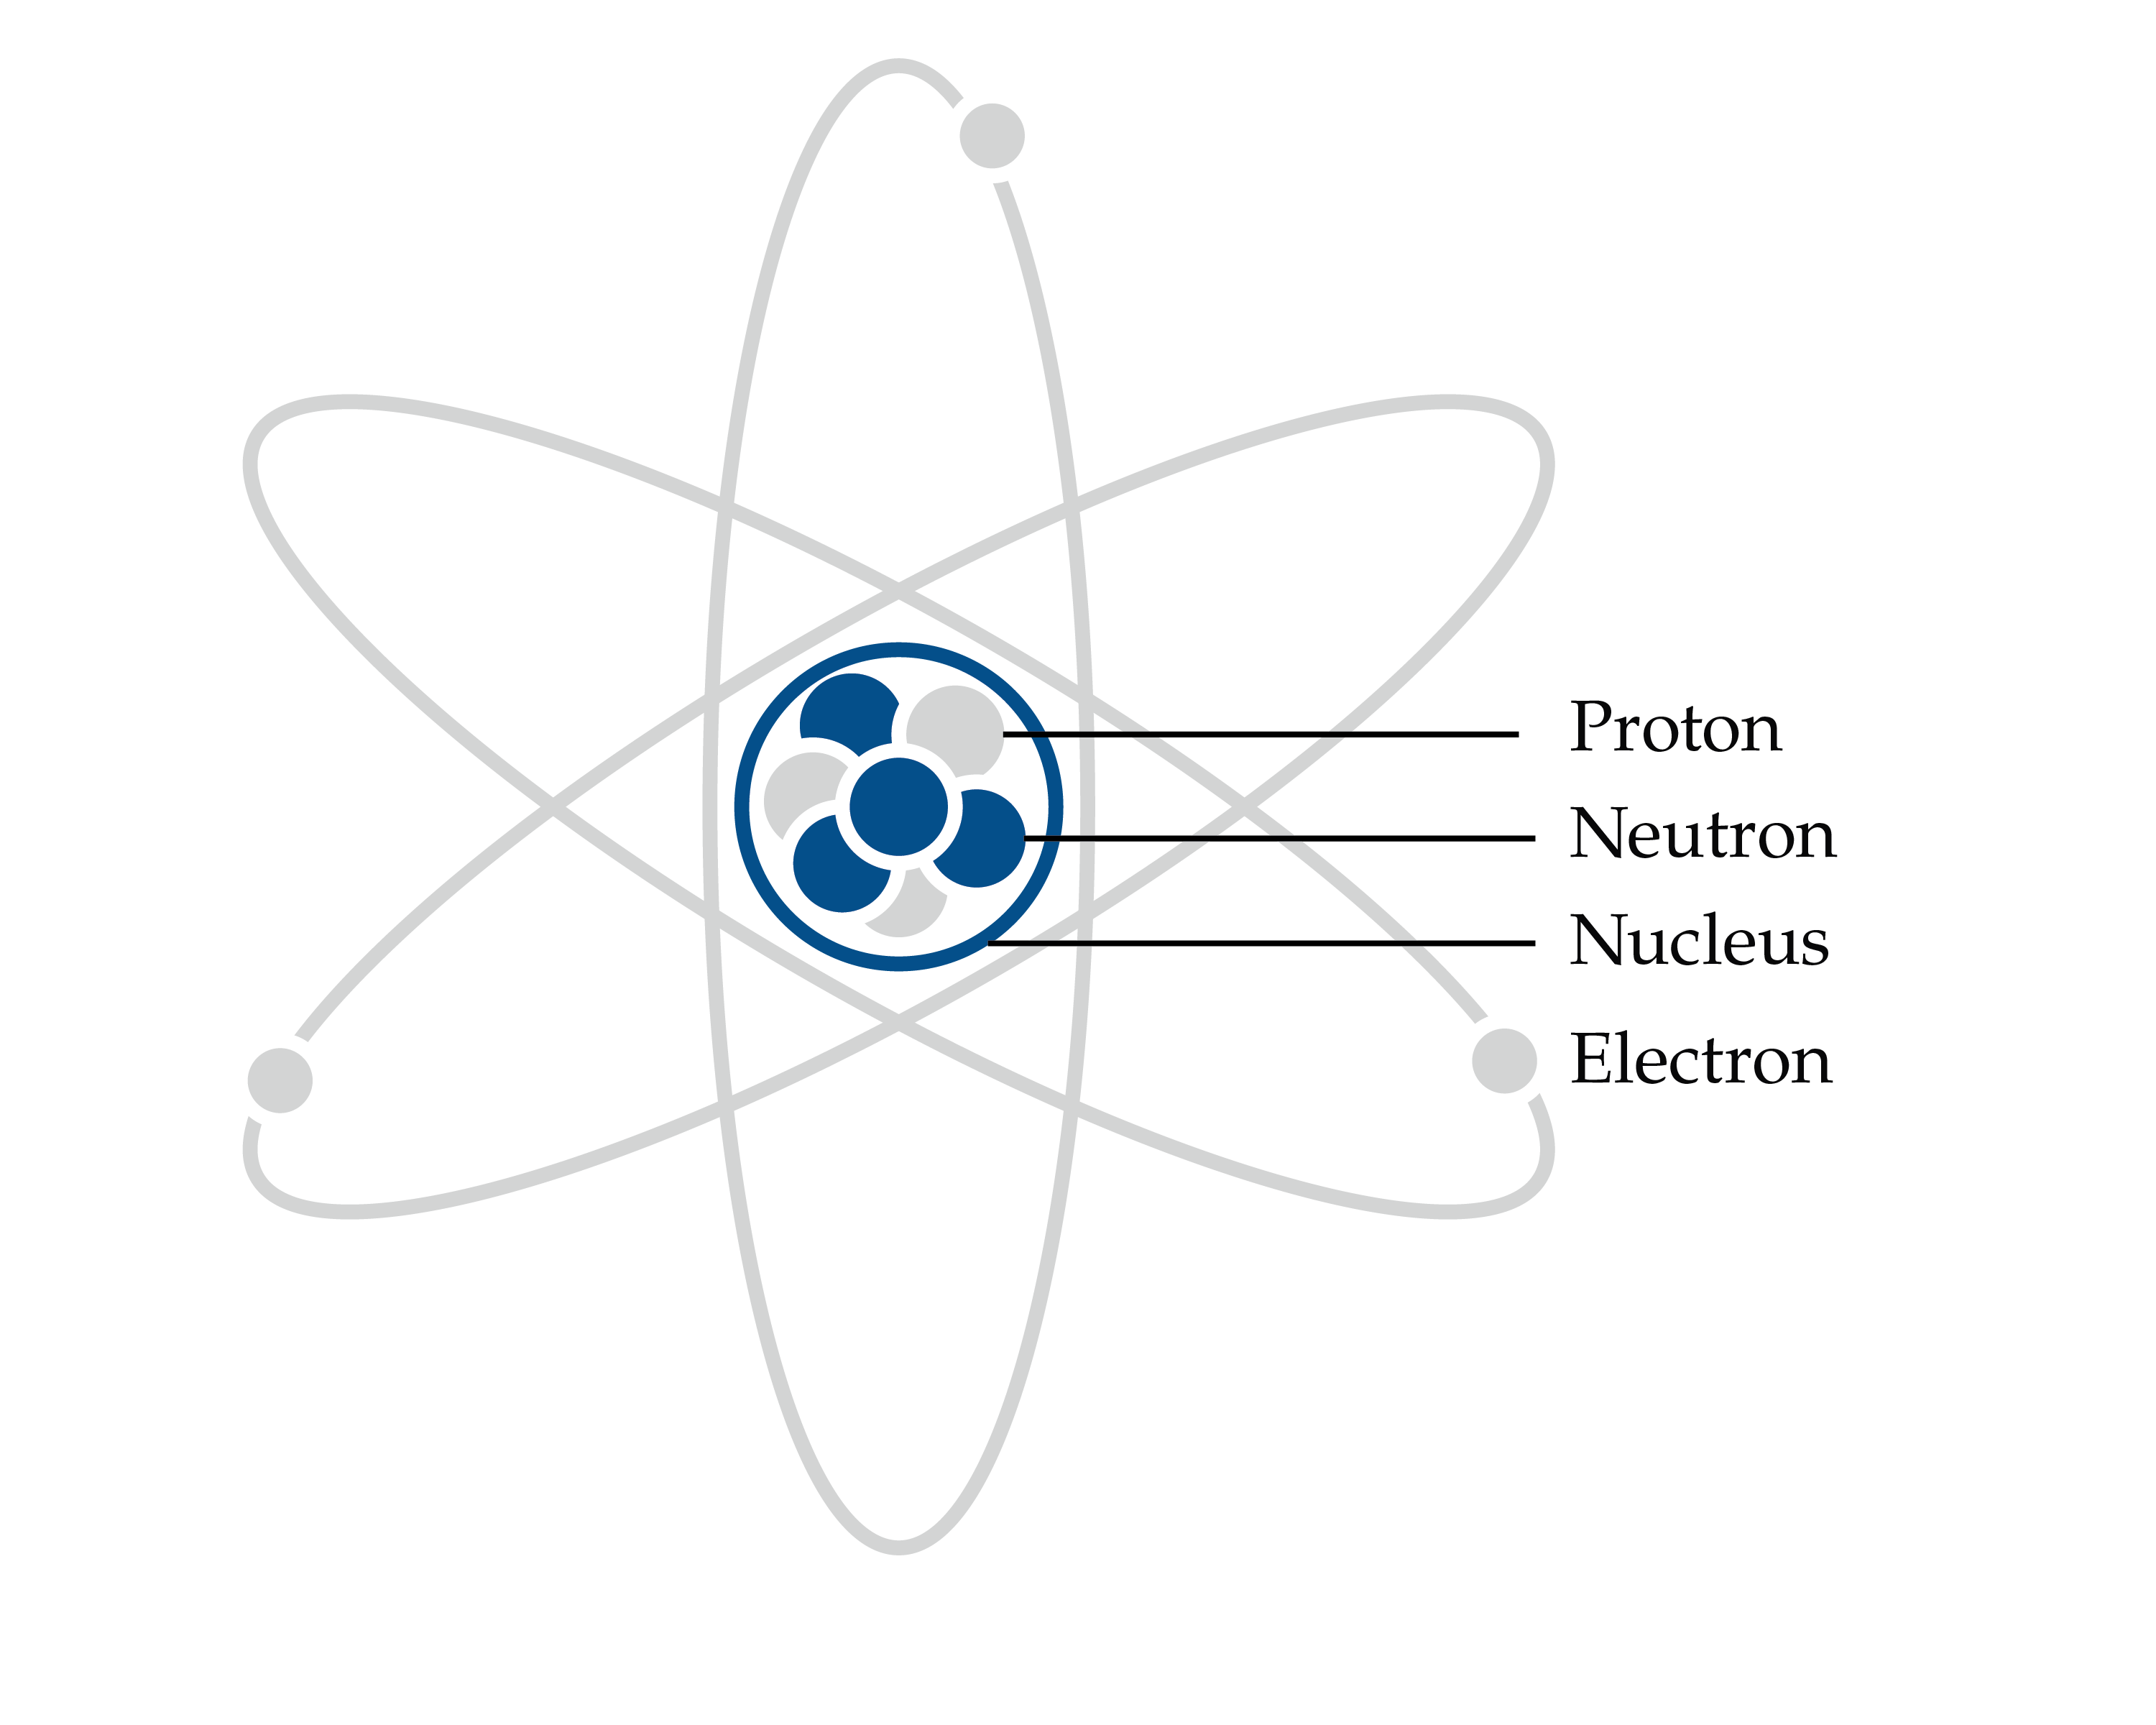
\includegraphics[width=.5\textwidth]{atom1.png}

Watch \textbf{Elements and atoms} from Khan Academy at \url{https://youtu.be/IFKnq9QM6_A}.

% ADD: Maybe get into different representaions of the atom: plum pudding, nuclear, planetary, quantum 

We classify atoms by the numbers of protons they have. An atom with one proton is a
hydrogen atom, an atom with two protons is a helium atom, and so forth (refer to periodic table on pg..). We say that hydrogen and helium are

\textit{elements} because the classification of elements is based on proton number. And we give
each element an atomic symbol. Hydrogen gets $H$. Helium gets $He$ Oxygen gets
$O$. Carbon gets $C$\index{elements}, etc.

Often two hydrogen atoms will attach to an oxygen atom. The result is
a water molecule. Why do they cluster together? because they share 
electrons in their clouds.\index{molecules}
% ADD:Electronegativity

A molecule is described by the elements it contains. Water is $H_2O$
because it has two hydrogen atoms and one oxygen atom.

There are many kinds of molecules. You know a few:
\begin{itemize}
\item Table salt is crystals made of $NaCl$ molecules: a sodium atom attached to a chlorine atom.
\item Baking soda, or sodium bicarbonate, is $NaHCO_3$.
\item Vinegar is a solution including acetic acid ($CH_3COOH$).
\item $O_2$ is the oxygen molecules that you breathe out of the air (Air, a blend of gases, is mostly $N_2$.).
\end{itemize}


Sometimes two hydrogen atoms form a molecule ($H_2$). Sometimes two
oxygen atoms form a molecule ($O_2$). If you mix these
together and light a match, they will rearrange themselves into water
molecules. This is called a \textit{chemical reaction}.  In any
chemical reaction, the atoms are rearranged into new molecules.\index{chemical reaction}
% ADD: electronegativity

Some chemical reactions (like the burning of hydrogen gas described
above) are \textit{exothermic} -- that is, they give off energy.
Burning hydrogen gas happens quickly and gives off a lot of energy. If
you have enough, it will make quite an explosion.\index{exothermic}
% ADD: endo/ exo thermic graphs/ explination

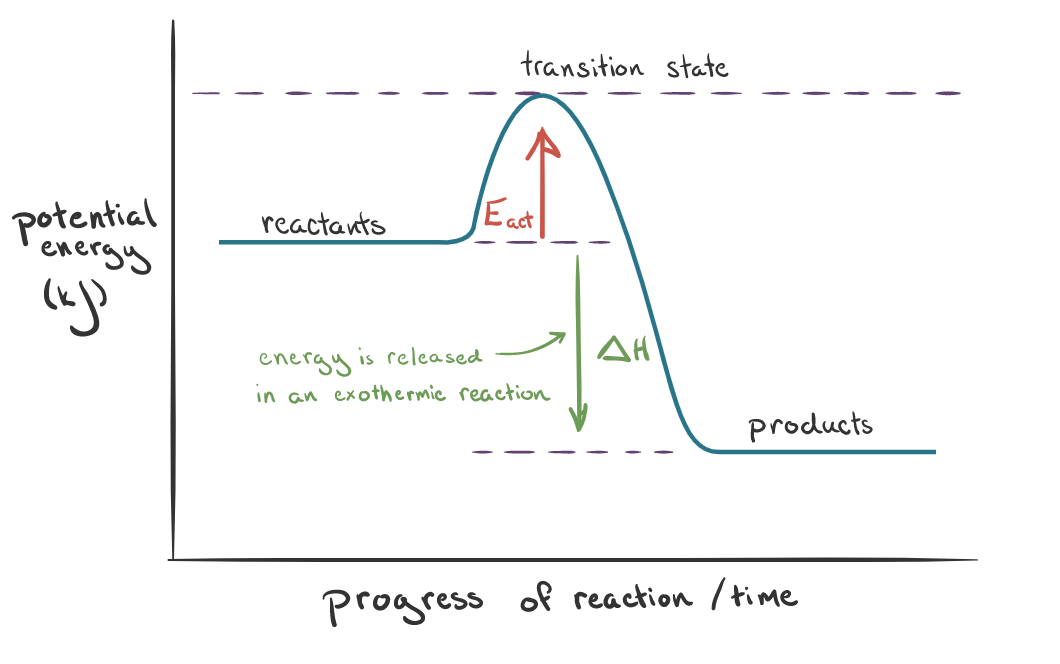
\includegraphics[width=0.7\textwidth]{KA_Exo.png}

Other chemical reactions are \textit{endothermic} -- that is they consume
energy.  Photosynthesis, the process by which plants consume energy
from the sun to make sugar from $CO_2$ and $H_2O$ requires an endothermic
chemical reaction.\index{endothermic}

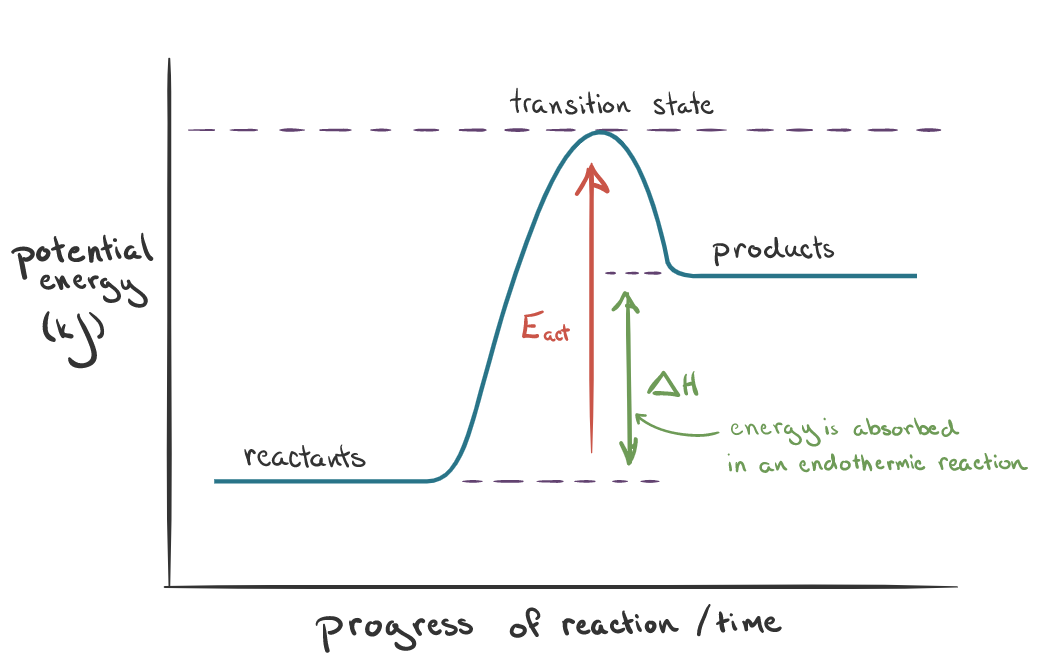
\includegraphics[width=0.7\textwidth]{KA_Endo.png}

\section{Mass and Acceleration}

Each atom has a mass, so everything that is made up of atoms has a
mass, which is pretty much everything.  We measure mass in grams.  A
paper clip is about 1 gram of steel. An adult human can weigh 70,000
grams, so for larger things we often talk about kilograms. A kilogram
is 1000 grams.

The first interesting thing about mass is that objects with more mass
require more force to accelerate. For example, pushing a bicycle so
that it accelerates from a standstill to jogging speed in 2 seconds
requires a lot less force than pushing a train so that it accelerates
at the same rate.

You will probably find it useful to watch Khan Academy's summary of
Newton's second law of motion: \url{https://youtu.be/ou9YMWlJgkE}

\begin{mdframed}[style=important, frametitle={Newton's Second Law of Motion}]

The force necessary to accelerate an object of mass $m$ is given by:

$$F = m a$$

That is the force is equal to the mass times the acceleration.

\end{mdframed}

What are the units here? We already know that mass is measured in
kilograms. We can measure velocity in meters per second, but that is
different from acceleration. Acceleration is the rate of change in
velocity. So if we want to go from 0 to 5 meters per second (that's
jogging speed) in two seconds. That is a change in velocity of 2.5
meters per second every second. We would say this acceleration is $2.5
m/s^2$.

What about measuring force? Newton decided to name the unit after
himself: The force necessary to accelerate one kilogram at $1 m/s^2$
is known as \textit{a newton}.

\begin{Exercise}[title={Acceleration}, label=acceleration_train]
  
While driving a bulldozer, you come across a train car (with no brakes
and no locomotive) on a track in the middle of a city. The train car
has a label telling you that it weighs 2,400 kg. There is a bomb
welded to the interior of the train car, and the timer tells you that
you can safely push the train car for 120 seconds. To get the train
car to where it can explode safely, you need to accelerate it to 20 meters per
second. Fortunately, the track is level and the train car's wheels have
almost no rolling resistance.

With what force, in newtons, do you need to push the train for those 120 seconds?

\end{Exercise}
\begin{Answer}[ref=acceleration_train]
To get the train to 20 meters per second in 120 seconds, you must
accelerate it with a constant rate of $\frac{1}{6} m/s^2$. You
remember that $F = m a$, so $F = 2400 \times \frac{1}{6}$. Thus, you
will push the train with a force of 400 newtons for the 120 seconds
before the bomb goes off.
\end{Answer}

\section{Mass and Gravity}

The second interesting thing about mass is that masses are
attracted to each other by the force we call \textit{gravity}. The
force of attraction between two objects is proportional to the product
of their masses. As objects get farther away, the force decreases.
That is why you are more attracted to the earth than you are to
distant stars, which have much more mass than the earth.
%ADD: Collums Law

\begin{mdframed}[style=important, frametitle={Newton's Law of Universal Gravitation}]

Two masses ($m_1$ and $m_2$) that are a distance of
$r$ from each other, are attracted toward each other with a force of
magnitude:

$$F = G\frac{m_1 m_2}{r^2}$$

where $G$ is the universal gravitational constant. If you measure the
mass in kilograms and the distance in meters. $G$ is about $6.674
\times 10^{-11}$.  That will get you the force of the attraction in
newtons.

\end{mdframed}

\begin{Exercise}[title={Gravity}, label=gravity_earth]
  
  The earth's mass is about $6 \times 10^{24}$ kilograms.

  Your spacecraft's mass is 6,800 kilograms.

  Your spacecraft is also about 100,000 km from the center of the earth. (For reference, the moon is about 400,000 km from the center of the earth.)

  What is the force of gravity that is pulling your spacecraft and the earth toward each other?

\end{Exercise}
\begin{Answer}[ref=gravity_earth]

  $$F = G\frac{m_1 m_2}{r^2} = (6.674 \times 10^{-11})\frac{(6.8 \time 10^3)(6 \times 10^{24})}{(10^5)^2} = 6.1 \times 10^{6}$$

  About 6 million newtons.
  
\end{Answer}

\section{Mass and Weight}

Gravity pulls on things proportional to their mass, so we often
ignore the difference between mass and weight.

The weight of an object is the force due to the object's mass and
gravity.  When we say, ``This potato weighs 1 pound,'' we actually mean
``This potato weighs 1 pound on earth.''  That same potato would weigh
about one-fifth of a pound on the moon.

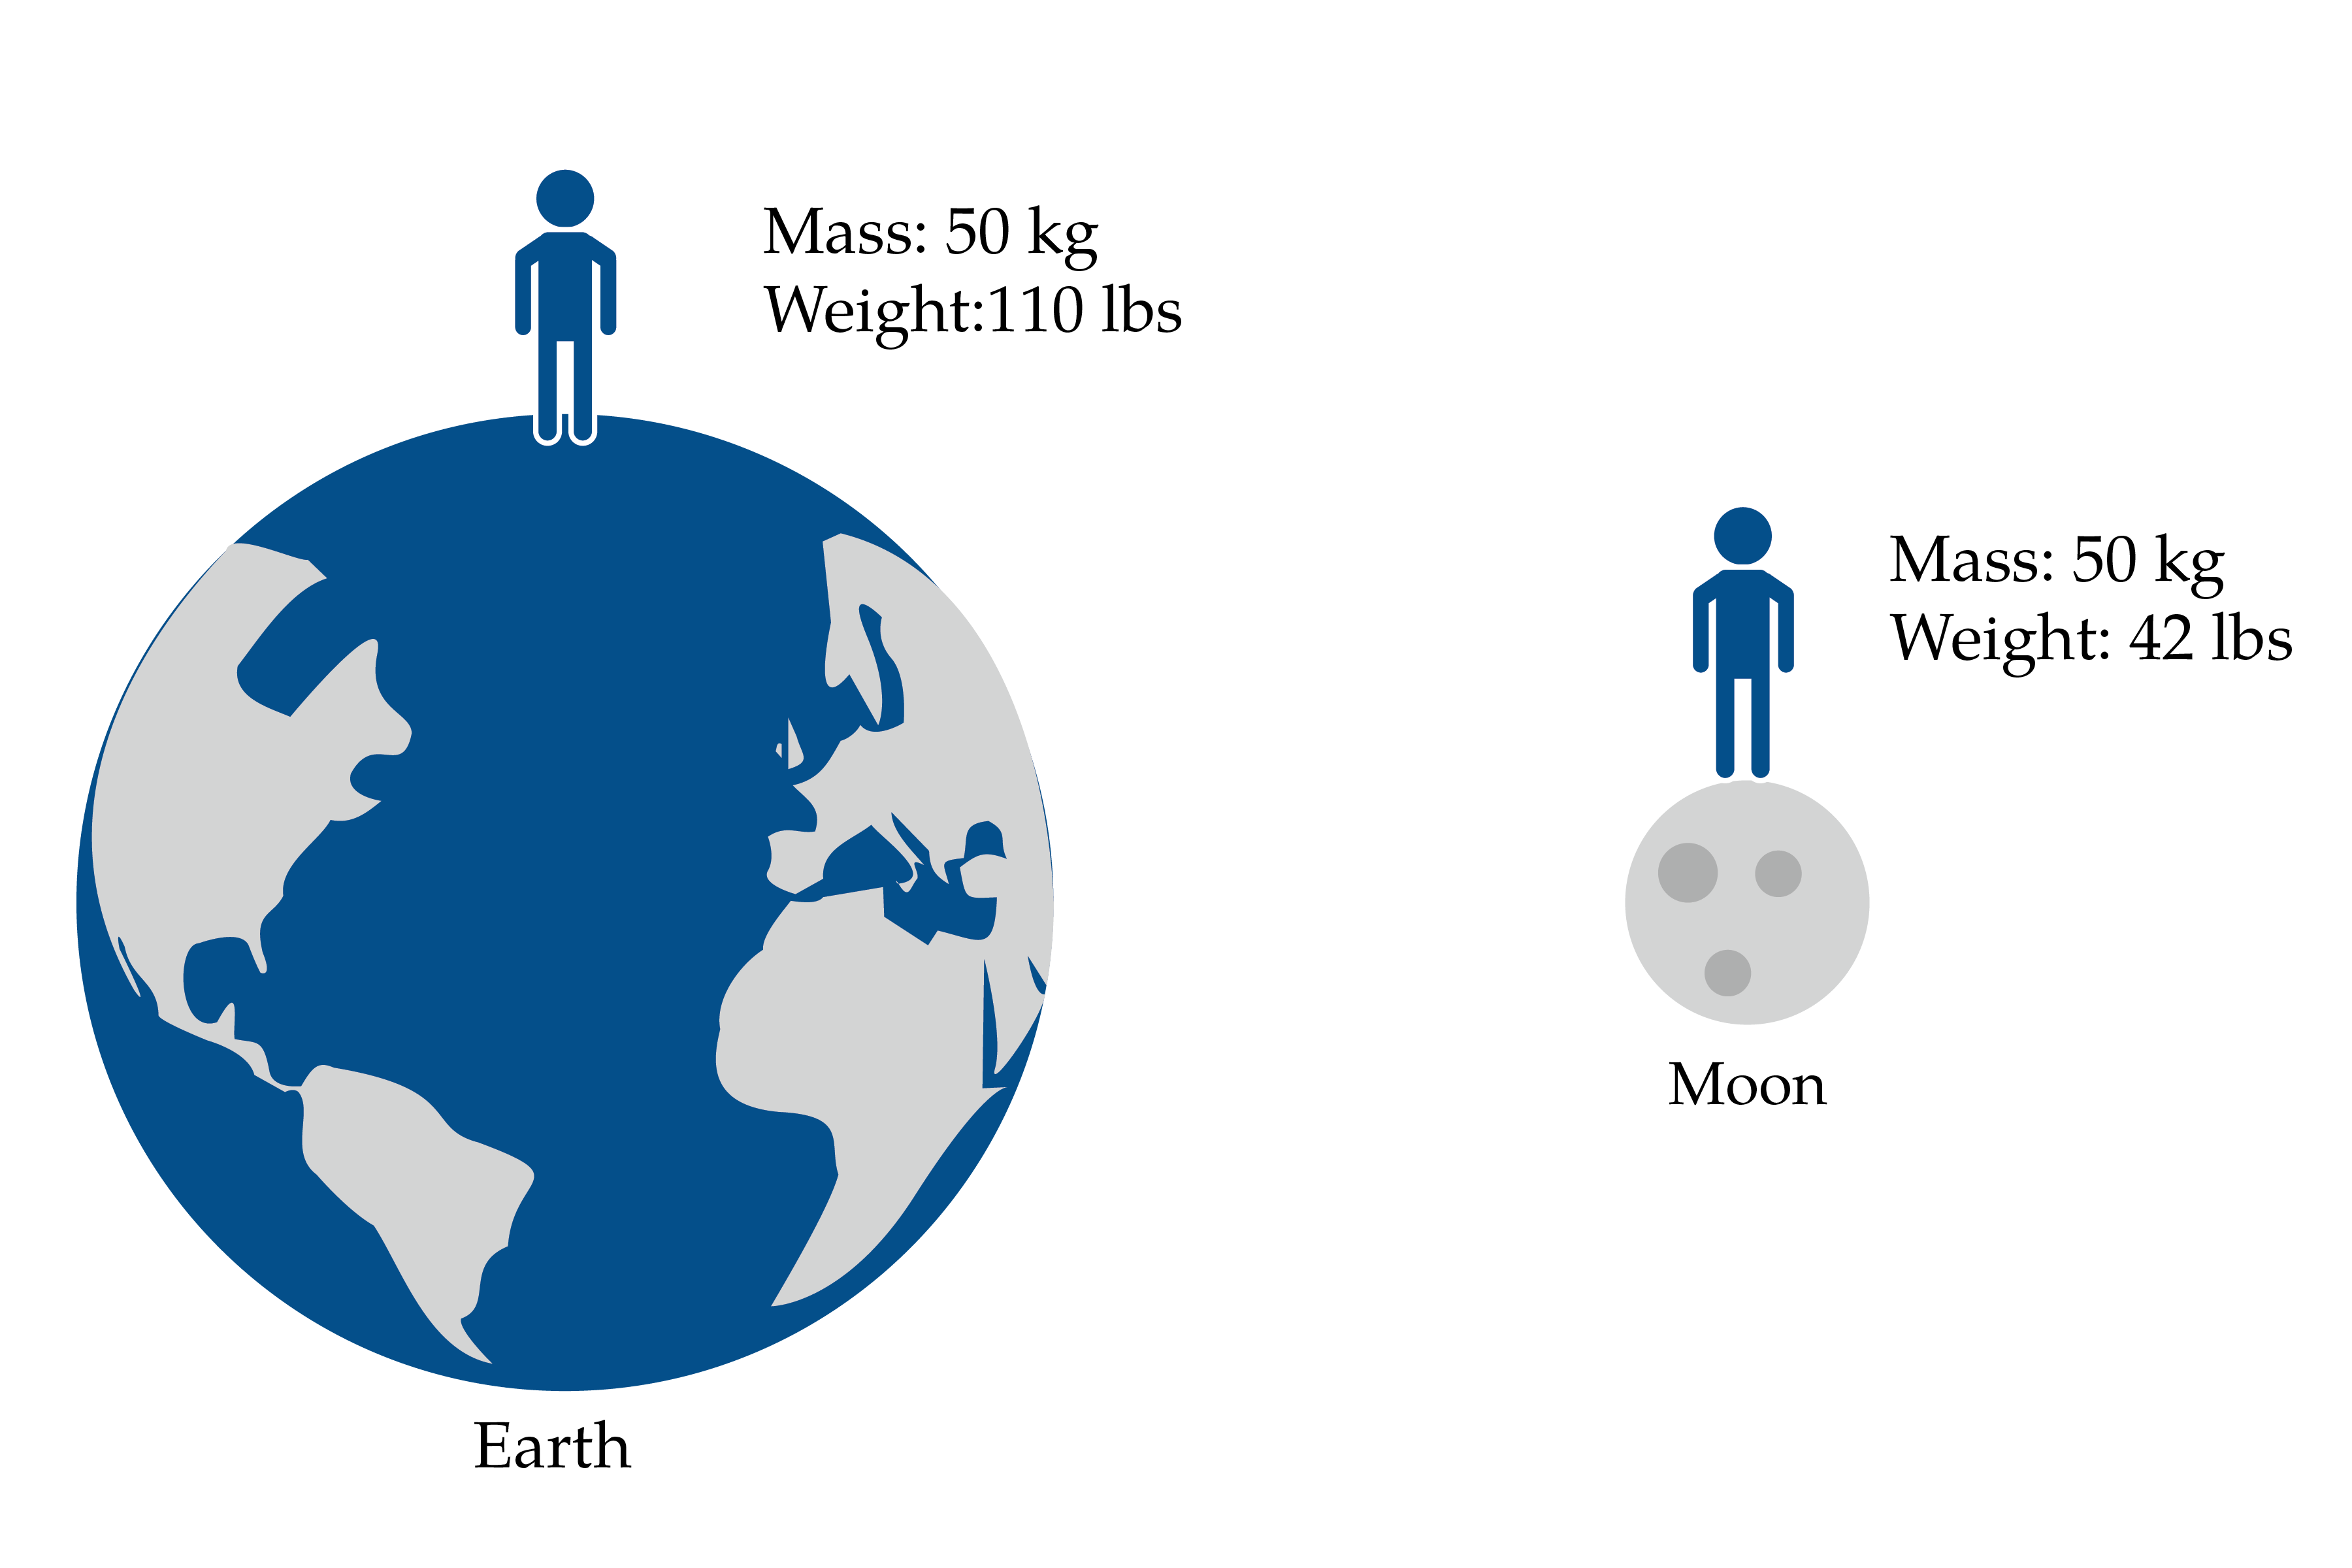
\includegraphics[width=0.6\textwidth]{massvweight.png}

But that potato has a mass of 0.45 kg anywhere in the universe.

\graphicspath{{../../Chapters/atomic_mass/en_US}}
\chapter{Atomic and Molecular Mass}

A proton and a neutron have about the same mass. An electron, on the
other hand, has much less mass: One neutron weighs about the same
amount as 2000 electrons. Thus, the mass of any object comes mostly
from the protons and neutrons in the nucleus of its atoms.\index{proton} \index{neutron}

We know how many protons an atom has by what element it is, but how do we know the number neutrons?

If you buy a balloon filled with helium, it will have two different
kinds of helium atoms: Most of the helium atoms will have 2 neutrons, but a
few will have only 1 neutron. We say that these are two different
\textit{isotopes} of helium. We call them helium-4 (or $^4He$) and
helium-3 (or $^3He$).  Isotopes are named for the sum of protons and
neutrons the atom has: helium-3 has 2 protons and 1 neutron.\index{isotopes}

Watch Khan Academy's \textbf{Atomic mass, number, and isotopes} at \url{https://www.khanacademy.org/science/chemistry/atomic-structure-and-properties/introduction-to-the-atom/v/atomic-number-mass-number-and-isotopes}

A hydrogen atom nearly always has just 1 proton and no neutrons. A
helium atom nearly always has 2 protons and 2 neutrons. So, if you
have a 100 hydrogen atoms and 100 helium atoms, the helium will have
about 4 times more mass than the hydrogen. We say ``Hydrogen is about
1 atomic mass unit(amu), and helium-4 is about 4 atomic mass
units.''\index{atomic mass unit}

What, precisely, is an atomic mass unit? It is defined as 1/12 of
the mass of a carbon-12 atom. Scientists have measured the mass of
helium-4, and it is about 4.0026 atomic mass units. (By the way, an
atomic mass unit is also called a \textit{dalton}.)

\pagebreak

Now you are ready to take a good look at the periodic table of
elements. Here is the version from Wikipedia:\index{periodic table of elements}

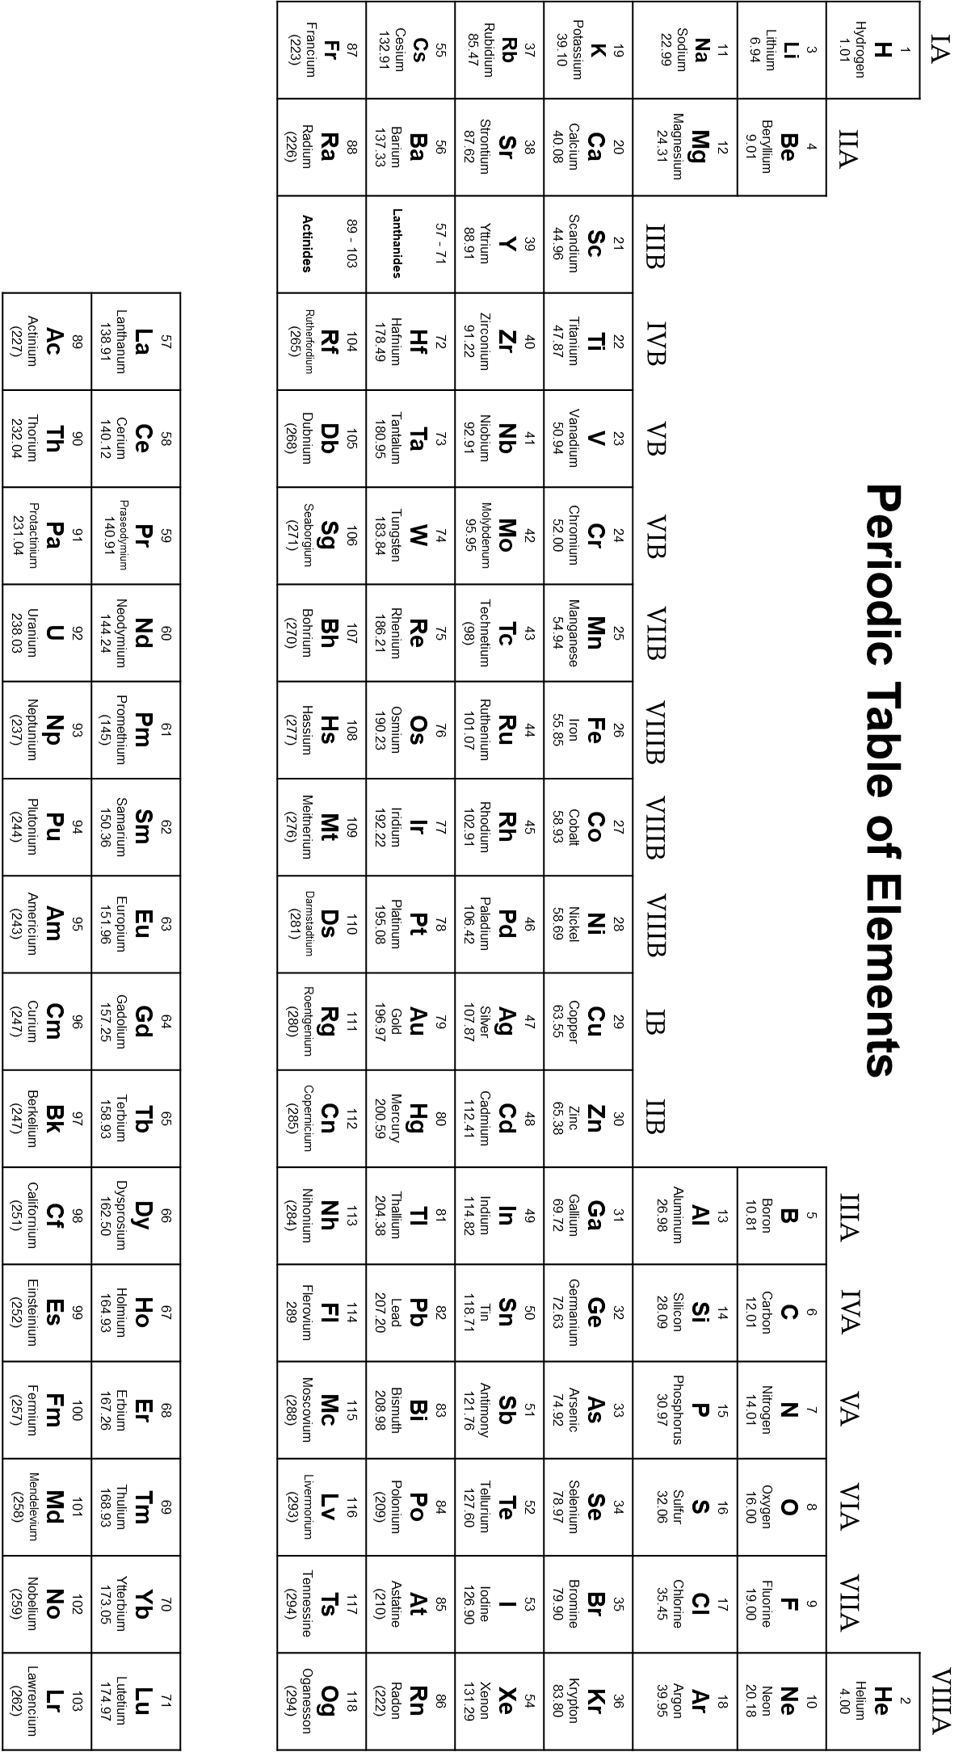
\includegraphics[width=0.75\textwidth]{periodic.png}

% ADD: Periodic Trends, Periods, Collums, Atomic Radius, Electronegativity,

\pagebreak
There is a square for each element. In the middle, you see the atomic
symbol and the name of the element. In the upper right corner is the
atomic number -- the number of protons in the atom.

In the upper left corner is the atomic mass in atomic mass units.\index{atomic mass}

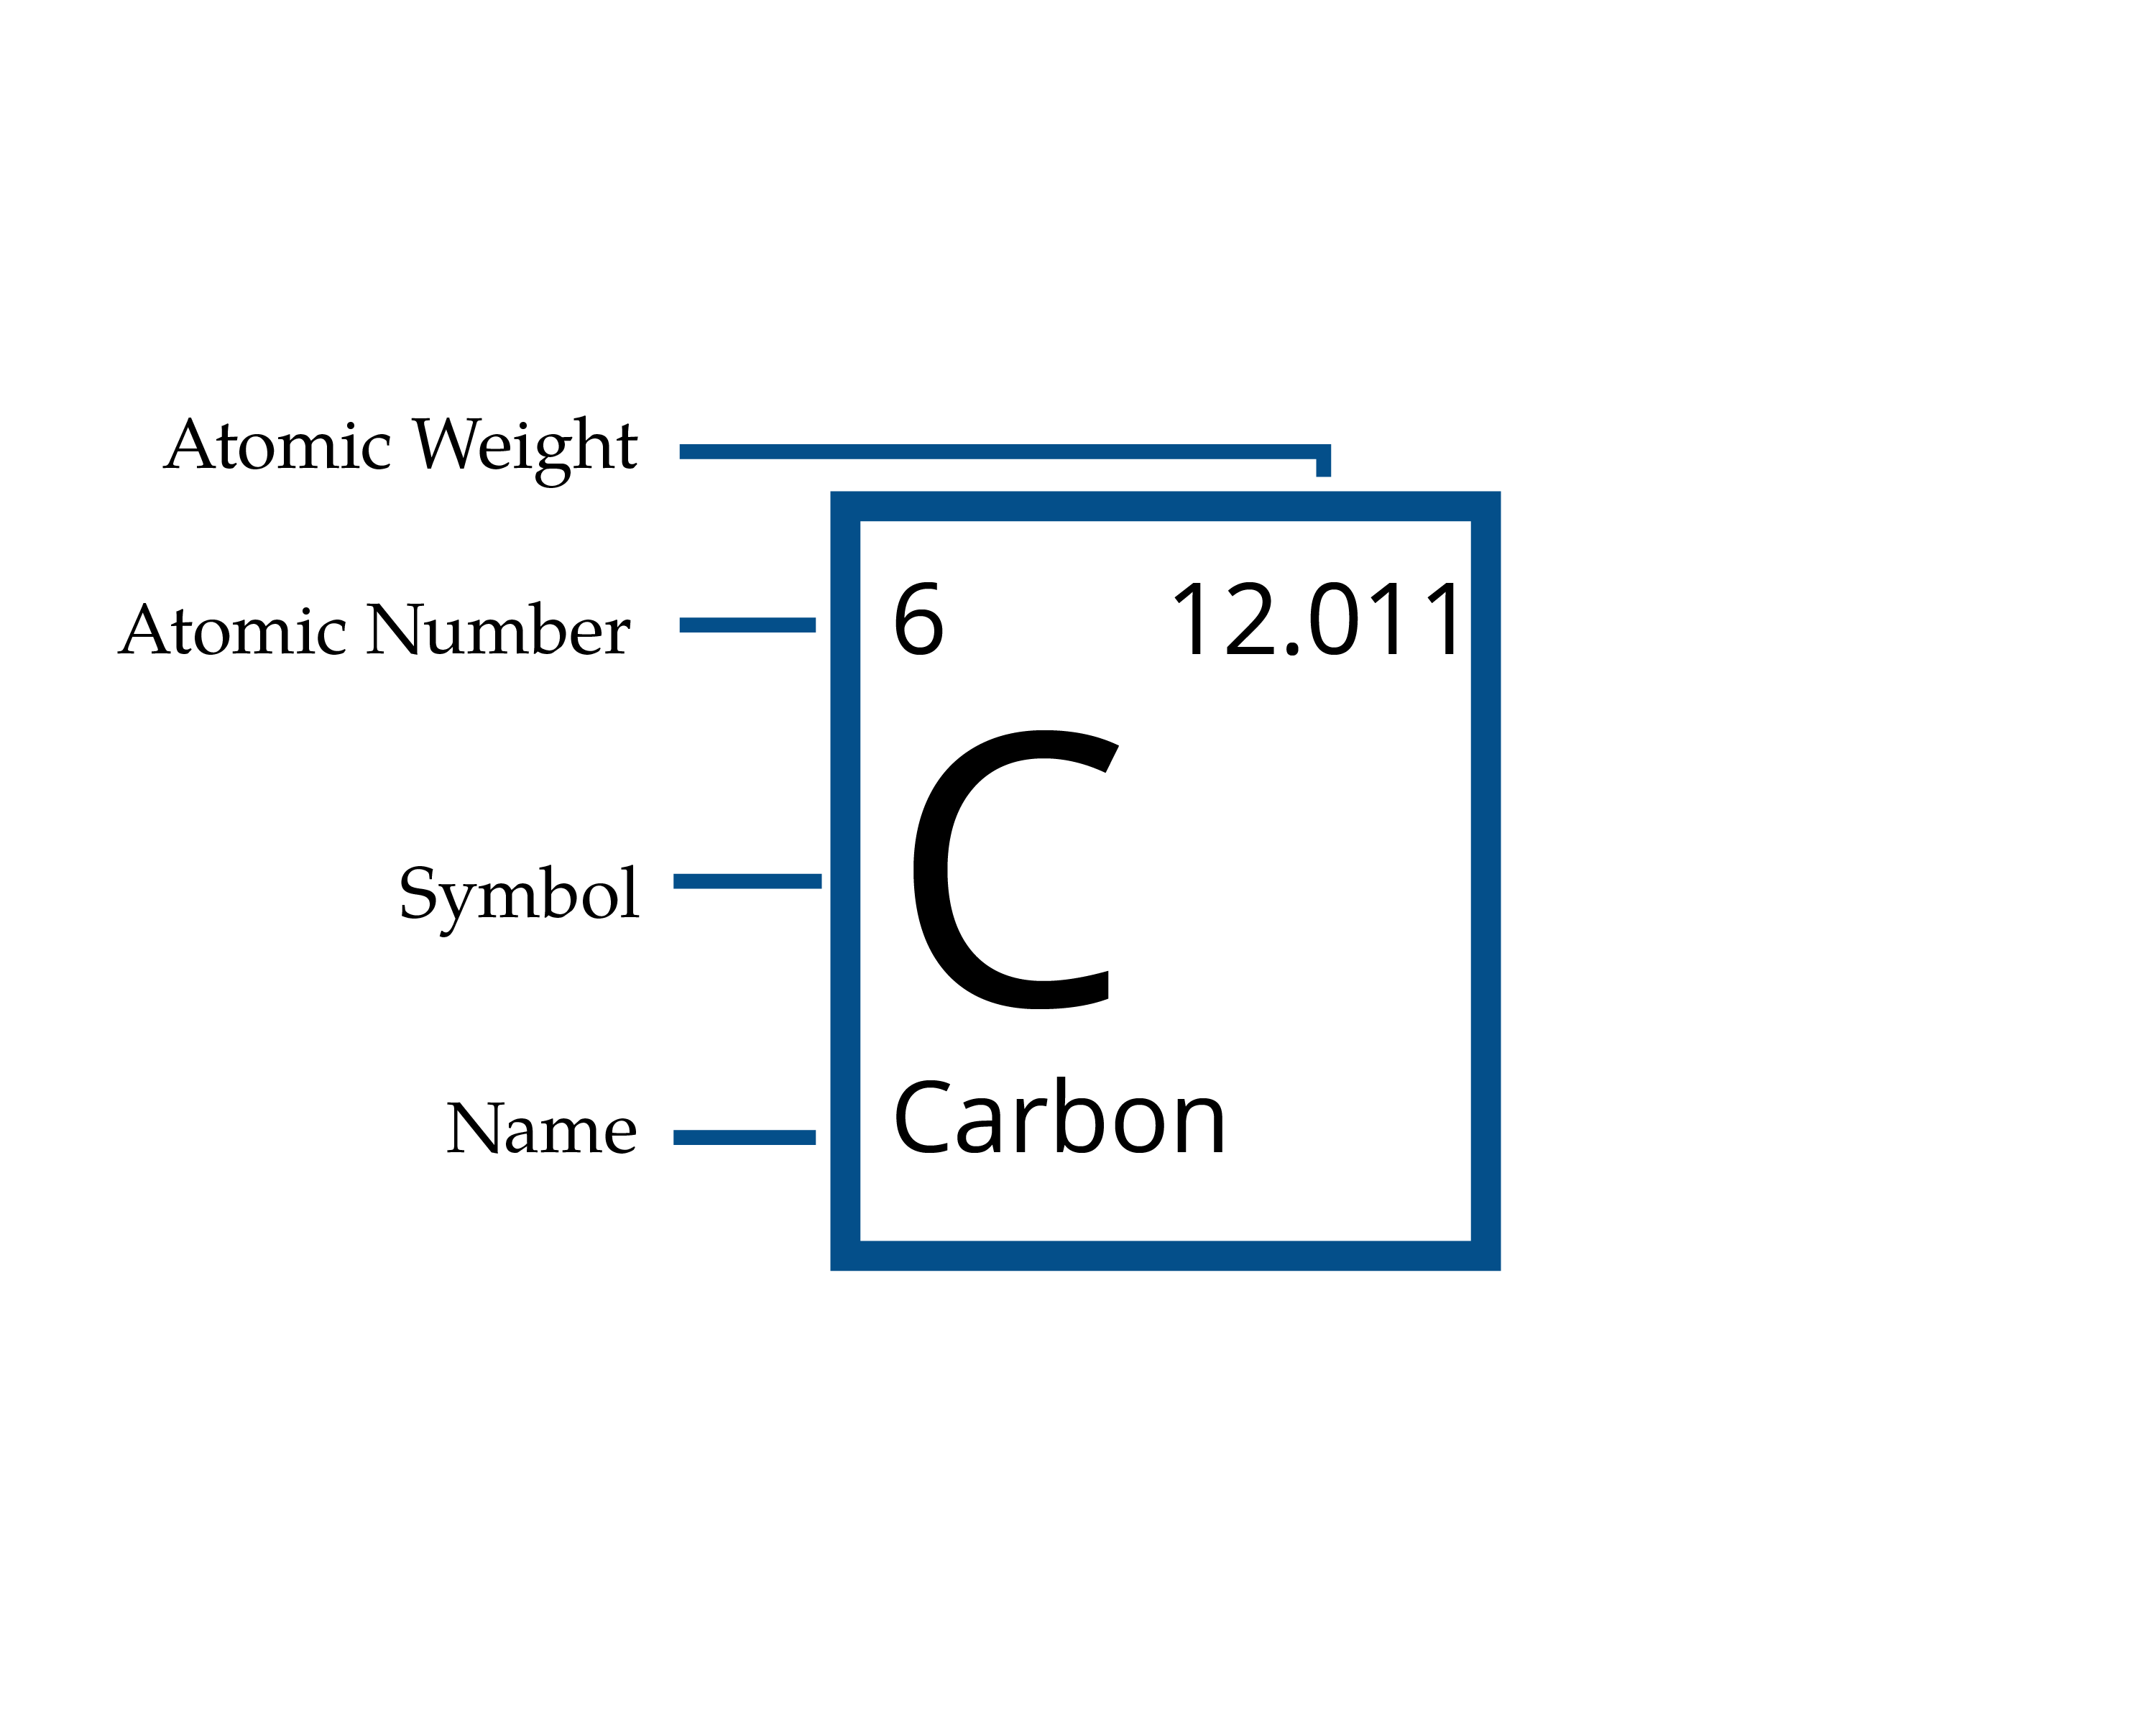
\includegraphics[width=0.8\textwidth]{element.png}

Look at the atomic mass of boron. About 80\% of all boron atoms have
six neutrons. The other 20\% have only 5 neutrons. So most boron atoms
have a mass of about 11 atomic mass units, but some have a mass of
about 10 atomic mass units. The atomic mass of boron is equivalent to the average
mass of a boron atom: 10.811.
% ADD: Talk about mass spectroscopy
%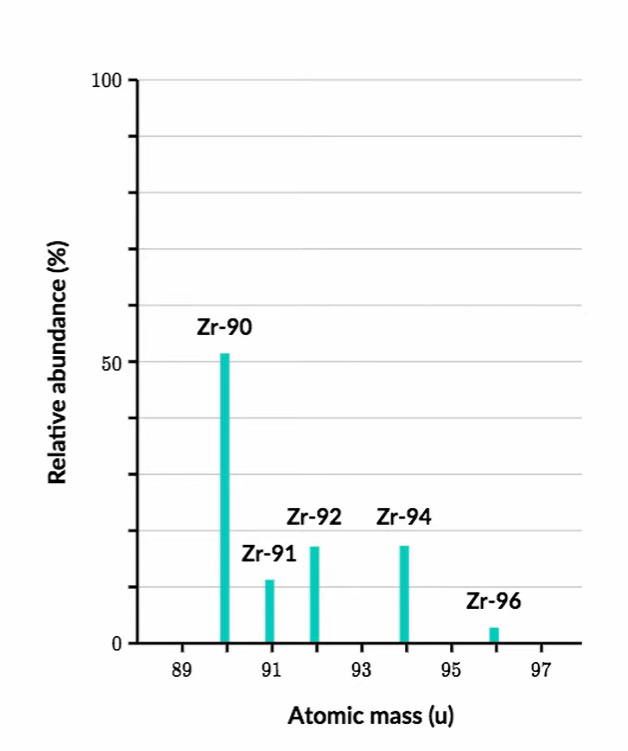
\includegraphics[width=0.75\textwidth]{KA_Mass_Spectroscopy_Zr.png}

\begin{Exercise}[title={Mass of a Water Molecule}, label=water_mass]
  
Using the periodic table, what is the average mass of one water molecule in atomic mass units?

\end{Exercise}
\begin{Answer}[ref=water_mass]

  The average hydrogen atom has a mass of 1.00794 atomic mass units.

  The average oxygen atom has a mass of 15.9994.

  $2 \times 1.00794 + 15.9994 = 18.01528$ atomic mass units.
   
\end{Answer}

\section{Molar Mass}

An atomic mass unit is a very, very, very small unit; we would much
rather work in grams.  It turns out that $6.02214076 \times 10^{23}$
atoms equal 1 mole( a standard measure for chemistry). Scientists use this number so much
that they gave it a name: \textit{the Avogadro constant} or
\textit{Avogadro's number}.\index{Avogadro's number}

Watch Khan Academy's discussion of the mole at \url{https://www.khanacademy.org/science/ap-chemistry-beta/x2eef969c74e0d802:atomic-structure-and-properties/x2eef969c74e0d802:moles-and-molar-mass/v/the-mole-and-avogadro-s-number}

If you have 12 doughnuts, that's a dozen doughnuts.  If you have
$6.02214076 \times 10^{23}$ doughnuts, you have a \textit{mole} of
doughnuts. (Note: it isn't practical to measure doughnuts this
way: A mole of doughnuts would be about the size of the earth. We use
moles for small things like molecules.)\index{mole}

Let's say you want to know how much a mole of $NaCl$ weighs. From the
periodic table, you see that $Na$ has an atomic mass of 22.98976
atomic mass units. And $Cl$ has 35.453 atomic mass units.  One atom of
$NaCl$ has a mass of $22.98976 + 35.453 = 58.44276$ atomic mass units.
Then a mole of $NaCl$ has a mass of $58.44276$ grams. Handy, right?
% ADD: Conversions should probably come before this

\begin{Exercise}[title={Burning Methane}, label=burning_methane]
  
Natural gas is mostly methane ($CH_4$). When one molecule of methane
burns, two oxygen molecules ($O_2$) are consumed. One molecule of
$H_2O$ and one molecule of $CO_2$ are produced.
% ADD: Need to explain mole to mole ratios first, Law of Divine Proportion
% ADD: Include Significant Figures

If I need 200 grams of water, how many grams of methane do I need
to burn?

(This is how the hero in ``The Martian'' made water for his garden.)

\end{Exercise}
\begin{Answer}[ref=burning_methane]

From the last exercise, you know that 1 mole of water weighs 18.01528
grams. So 200 grams of water is about 11.1 moles. So you need to burn
11.1 moles of methane.

What does one mole of methane weigh? Using the periodic table:
$12.0107 + 4 \times 1.00794 = 16.04246$ grams.

$16.0424 \times 11.10 = 178.1$ grams of methane.
   
\end{Answer}

\section{Heavy atoms aren't stable}

When you look at the periodic table, there are a surprisingly large
number of elements. You might be told to ``Drink milk so that you can
get the calcium you need.'' However, no one has told you ``You should
eat kale so that you get enough copernicium in your diet.''

Copernicium, with 112 protons and 173 neutrons, has only been observed
 in a lab. It is highly radioactive and unstable(meaning it decays): a copernicium
atom usually lives for less than a minute before decaying.
% ADD: Half Life

The largest stable element is lead, which has 82 protons and between
122 and 126 neutrons. Elements with lower atomic numbers than lead,
have at least one stable isotope. Elements with higher atomic numbers
than lead don't.

Bismuth, with an atomic number of 83, is \textit{almost} stable. In fact, most
bismuth atoms will live for billions of years before decaying.

\graphicspath{{../../Chapters/work_energy/en_US}}
\chapter{Work and Energy}

In this chapter, we are going to talk about how engineers define work
and energy.  We have already talked about force. Force is measured in
newtons, and one newton is equal to the force necessary to accelerate one
kilogram at a rate of $1 m/s^2$.

When you lean on a wall, you are exerting a force on the wall, but you
aren't doing any work. On the other hand, if you push a car for a mile,
you are clearly doing work. Work, to an engineer, is the force you
apply to something, as well as the distance that it moves, in the direction
of the applied force. We measure work in \textit{joules}. A joule is one
newton of force over one meter.\index{Joule}

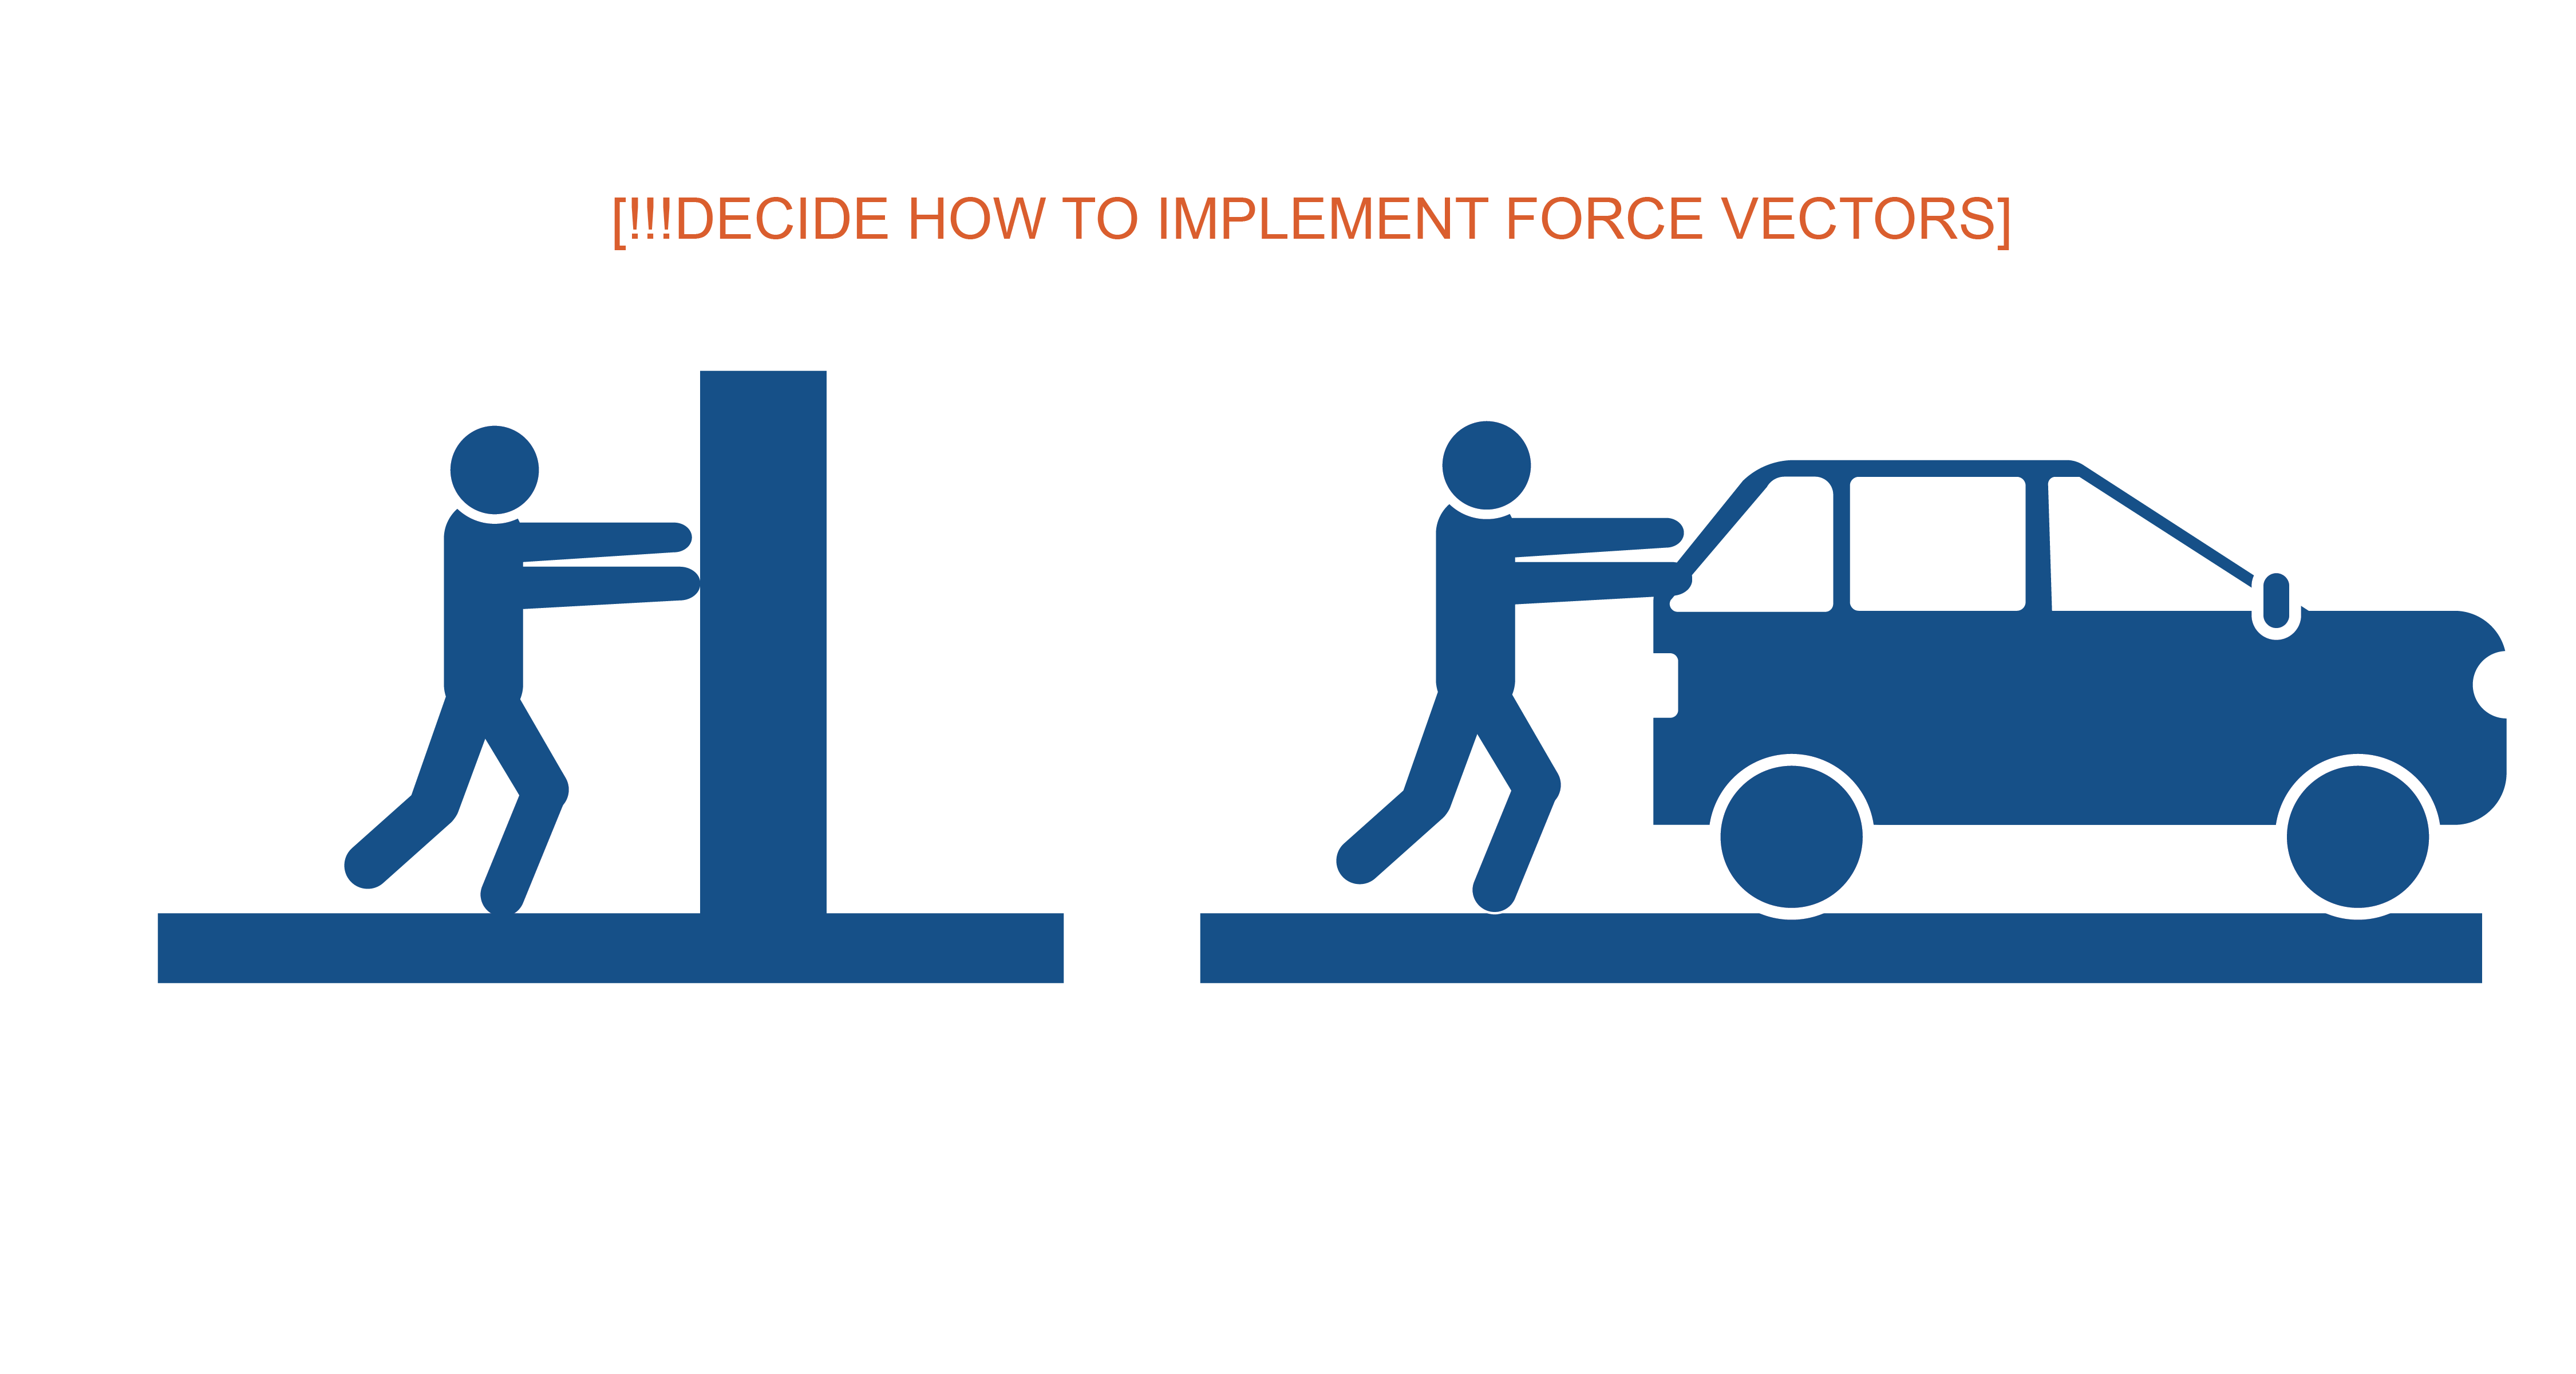
\includegraphics[width=0.5\textwidth]{workvsforce.png}

For example, if you push a car uphill with a force of 10 newtons for 12
meters, you have done 120 joules of work.\index{work}
% ADD: We can represent this with the equations, Work Energy Therom

Work is how energy is transferred from one thing to another. When you
push the car, you also burn sugars(energy of the body) in your blood. That energy is then
transferred to the car: after it has been pushed uphill.

Thus, we measure the energy something consumes or generates in 
units of work: joules, kilowatt-hours, horsepower-hours, foot-pounds,
BTUs( British Thermal Unit), and calories.

Let's go over a few different forms that energy can take.

Watch Khan Academy's \textbf{Changes in energy} at \url{https://www.khanacademy.org/science/ms-physics/x1baed5db7c1bb50b:energy/x1baed5db7c1bb50b:changes-in-energy/a/changes-in-energy}

\section{Heat}\index{heat}

When you heat something, you are transferring energy to it. The BTU
 is a common unit for heat: One BTU is the
amount of heat required to raise the temperature of one pound of water,
by one degree. One BTU is about 1,055 joules. In fact, when you buy and sell
natural gas as fuel, it is priced by the BTU.\index{heat} \index{BTU}

\section{Electricity}\index{electricity}

Electricity is the movement of electrons. When you push electrons
through a space that resists their passage (like a light bulb),
energy is transferred from the power source ( a battery)
 into the source of the resistance.

Let's say your lightbulb consumes 60 watts of electricity, and you leave it on for 24 hours.
We would say that you have consumed 1.44 kilowatt hours or 3,600,000 joules.

Watch Khan Academy's \textbf{Introduction to charge} at \url{https://www.khanacademy.org/science/in-in-class10th-physics/in-in-electricity/in-in-electric-current-circuit/v/intro-to-charge}

\section{Chemical Energy}\index{chemical energy}

As mentioned early, some chemical reactions consume energy and some
produce energy. Thus, energy can be stored in the structure of a
molecule. When a plant uses photosynthesis to rearrange water and
carbon dioxide into a sugar molecule, it converts the energy in
the sunlight( solar energy) into chemical energy. Remember photosythesis is a process that releases energy.
Therefore, the sugar molecule has more chemical energy than the carbon dioxide and water molecules that were
used in its creation.
% ADD: photosythesis equation 
% KA: https://www.khanacademy.org/science/ap-biology/cellular-energetics/photosynthesis/a/intro-to-photosynthesis

In our diet, we measure this energy in \textit{kilocalories}. A
calorie is the energy necessary to raise one gram of water one degree
Celsius: it is about 4.19 joules. This is a very small unit: an apple
has about 100,000 calories( 100 kilocalories), so people working with food started
measuring everything in kilocalories.\index{calories}
% ADD: Conversion chapter should come before this chapter

Here is where things get confusing: People who work with food got tired of
saying ``kilocalories'', so they just started using ``Calorie'' to
mean 1,000 calories.  This has created terrible confusion over the
years. So if the C is capitalized, ``Calorie'' probably means kilocalorie.

\section{Kinetic Energy}\index{kinetic energy}

A mass in motion has energy. For example, if you are in a moving car
and you slam on the breaks, the energy from the motion of the
car will be converted into heat in the breaks and under the tires.

How much energy does the car have?
% ADD: section specifically about KE AND U, use roller coaster diagram

\begin{mdframed}[style=important, frametitle={Formula for Kinetic Energy}]

$$E = \frac{1}{2} m v^2$$

where $E$ is the energy in joules, $m$ is the mass in kilograms, and
$v$ is the speed in meters per second.

\end{mdframed}

\section{Gravitational Potential Energy}\index{potential energy!gravitational}

Watch Khan Academy's \textbf{Potential energy} at \url{https://youtu.be/oGzwVYPxKjg}

When you lift something heavy onto a shelf, you are giving it
\textit{potential energy}. The amount of energy that you transferred
to it is proportional to its weight and the height that you lifted it.

On the surface of the earth, gravity will accelerate a heavy object downward at
a rate of $9.8 m/s^2$.

\begin{mdframed}[style=important, frametitle={Formula for Gravitational Potential Energy}]
On earth, then, gravitational potential energy is given by

$$E = (9.8)mh$$


where $E$ is the energy in joules, $m$ is the mass of the object you
lifted, and $h$ is the height that you lifted it.

\end{mdframed}


There are other kinds of potential energy. For example, when you draw
a bow, you have given that bow potential energy. When you release it,
the potential energy is transferred to the arrow, which expresses it
as kinetic energy.
% ADD: section about KE and U

\section{Conservation of Energy}

The first law of thermodynamics says ``Energy is neither created nor
destroyed.''\index{energy!conservation of}

Energy can change forms: Your cells consume chemical energy to give
gravitational potential energy to a car you push up a hill. However, the total amount of
energy in a closed system stays constant.
% ADD: Create Systems chapter before introducing concept here

\begin{Exercise}[title={The Energy of Falling}, label=energy_falling]
  
A 5 kg cannonball falls off the top of a 3 meter ladder. Just before
it hits the floor, all of its gravitational potential energy has been
converted into kinetic energy.  How fast is the cannonball going when
it hits the floor?

\end{Exercise}
\begin{Answer}[ref=energy_falling]

  At the top of the ladder, the cannonball has $(9.8)(5)(3) = 147$ joules of potential energy.

  At the bottom, the kinetic energy $\frac{1}{2}(5)v^2$ must be equal
  to 147 joules. So $v^2 = \frac{294}{5}$.  Thus it is going about
  $7.7$ meters per second.

  (Yes, a tiny amount of energy is lost to air resistance. For a dense
  object moving at these relatively slow speeds, this energy is
  neglible.)
  
\end{Answer}


\section{Efficiency}


Watch Khan Academy's \textbf{Laws of thermodynamics} at \url{https://www.khanacademy.org/science/ap-biology/cellular-energetics/cellular-energy/a/the-laws-of-thermodynamics}

Although energy is always conserved as it moves through different
forms, scientists aren't always that good at controlling it.\index{efficiency}

For example, a car engine consumes the chemical energy in gasoline. Only
about 20\% of the energy consumed is used to turn the wheels.  Most of
the energy is actually lost as heat. If you run a car for a while, the engine
gets very hot and the exhaust going out the tailpipe turns hot.

A human is about 25\% efficient. Most of the loss is in the heat produced
during the chemical reactions that turns food into motion.
% ADD: Cellular Respiration
 
In general, if you are trying to increase efficiency in any system,
the solution is usually easy to identify because heat is produced. Reduce heat, Increase efficiency.

Light bulbs are an interesting case. To get the light of a 60 watt
incandescent bulb, you can use an 8 watt LED or a 16 watt fluorescent
light. Thus, we say that the LED light is much more efficient: If you
run both, the incandescent bulb will consume 1.44 kilowatt-hours. The
LED will consume only 0.192 kilowatt-hours.

Besides light, the incandescent bulb is producing a lot of heat. If it
is inside your house, what happens to the heat? It warms your house.

In the winter, when you want light and heat, the incandescent bulb is
100\% efficient!

In the summer, if you are running the air conditioner, the
incandescent bulb is worse than just ``inefficient at making light'' --
it is actually counteracting the air conditioner! 


\graphicspath{{../../Chapters/units_conversions/en_US}}
\chapter{Units and Conversions}

At this point, you are working with a lot of units: grams for weight,
joules for energy, newtons for force, meters for distance, seconds for
time, etc. For each type of measurement, there are several different
units; for example, distance can be measured in feet, miles,
and light-years.

\begin{mdframed}[style=important, frametitle={Some Equalencies}]

\begin{tabular}{r | l}
  \hline
  \multicolumn{2}{c}{\textbf{Distance}}\\
  1 mile & 1.6093 kilometers \\
  1 foot & 0.3048 meters \\
  1 inch & 2.54 centimeters \\
  1 light-year & $9.461 \times 10^{12}$ kilometers\\
  \hline
  \multicolumn{2}{c}{\textbf{Volume}}\\
  1 milliliter & 1 cubic centimeter \\
  1 quart & 0.9461 liters \\
  1 gallon & 3.7854 liters \\
  1 fluid ounce & 29.6 milliliters \\
  \hline
  \multicolumn{2}{c}{\textbf{Mass}}\\
  1 pound & 0.4535924 kilograms\\
  1 ounce & 0.4535924 grams\\
  1 metric ton & 1000 kilograms \\
  \hline
  \multicolumn{2}{c}{\textbf{Force}}\\
  1 newton & 1 kilogram meter per sec$^2$\\
  \hline
  \multicolumn{2}{c}{\textbf{Pressure}}\\
  1 pascal & 1 newton per square meter \\
  1 bar & 0.98692 atmosphere \\
  1 pound per square inch & 6897 pascals \\
  \hline
  \multicolumn{2}{c}{\textbf{Energy}}\\
  1 joule & 1 newton meter \\
  1 calorie & 4.184 joules \\
  1 kilowatt-hour & $3.6 \times 10^{6}$ joules  \\
\end{tabular}\index{units table}

(You don't need to memorize these! Just remember that this page is here.)
% Suggest putting this in the front or back of the book, maybe create a print out

\end{mdframed}

In the metric system, prefixes are often used to express a multiple. Here are the common prefixes:\index{metric system!prefixes}

\begin{mdframed}[style=important, frametitle={Common Prefixes for Metric Units}]

\begin{tabular}{r | l}
giga  & $\times 10^{9}$\\
mega  & $\times 10^{6}$\\
kilo  & $\times 10^{3}$\\
milli  & $\div 10^{3}$\\
micro  & $\div 10^{6}$\\
nano  & $\div 10^{9}$\\
\end{tabular}

(These are worth memorizing. Here's a mnemonic: ``King Henery Doesn't Usually Drink Chocolate Milk.'')
\end{mdframed}

\section{Conversion Factors}

Here is a really handy trick to remembering how to do conversions
between units.\index{conversion factors}

Often, you will be given a table like the one above, and someone will ask you
``How many miles are in 0.23 light-years?''  You know that 1 mile = 1.6093
kilometers and that 1 light-year is $9.461 \times 10^{12}$ kilometers.
How do you do the conversion?

The trick is to treat the two parts of the equality as a fraction that equals 1.  That is, you think:

$$\frac{1 \text{ miles}}{1.6093 \text{ km}} = \frac{1.6093 \text{ km}}{1 \text{ miles}} = 1$$

and

$$\frac{1 \text{ light-years}}{9.461 \times 10^{12} \text{ km}} = \frac{9.461 \times 10^{12} \text{ km}}{1 \text{ light-years}} = 1$$

We call these fractions \textit{conversion factors}.

Now, your problem is

$$0.23 \text{ light-years} \times \textit{ Some conversion factors} = ? \text{ miles}$$

Note that when you multiply fractions together, things in the numerators can cancel with things in the denominator:

$$\left( \frac{31\pi}{47} \right) \left( \frac{11}{37\pi}\right) = \left(\frac{31\cancel{\pi}}{47}\right) \left( \frac{11}{37\cancel{\pi}}\right) = \left(\frac{31}{47} \right) \left( \frac{11}{37} \right)$$

When working with conversion factors, you will do the same with the units:

\begin{multline*}
  0.23 \text{ light-years} \left( \frac{9.461 \times 10^{12} \text{ km}}{1 \text{ light-years}} \right) \left( \frac{1 \text{ miles}}{1.6093 \text{ km}} \right) = \\
  0.23 \text{ \cancel{light-years}} \left( \times \frac{9.461 \times 10^{12} \text{ \cancel{km}}}{1 \text{ \cancel{light-years}}} \right) \left( \frac{1 \text{ miles}}{1.6093 \text{ \cancel{km}}}\right) = \frac{(0.23)(9.461 \times 10^{12})}{1.6093} \text{ miles}$$
\end{multline*}

\begin{Exercise}[title={Simple Conversion Factors}, label=simple_conversion_factors]

  How many calories are in 4.5 kilowatt-hours?
  
\end{Exercise}
\begin{Answer}[ref=simple_conversion_factors]

  $$4.5 \text{ \cancel{kWh}} \left( \frac{3.6 \times 10^{6} \text{ \cancel{joules}}}{1 \text{ \cancel{kWh}}} \right) \left( \frac{1 \text{ calories}}{4.184 \text{ \cancel{joules}}}\right) = \frac{(4.5)(3.6 \times 10^6)}{4.184} = 1.08 \times 10^6 \text {calories}$$
  
\end{Answer}

\section{Conversion Factors and Ratios}

Conversion factors also work on ratios.  For example, if you are told
that a bug is moving 0.5 feet every 120 milliseconds. What is that in
meters per second?

The problem then is

$$\frac{0.5 \text{ feet}}{120 \text{ milliseconds}} = \frac{\text{? m}}{second}$$

So you will need conversion factors to replace the ``feet'' with ``meters'' and to replace ``milliseconds'' with ``seconds'':

\begin{multline*}
\left(\frac{0.5 \text{ \cancel{feet}}}{120 \text{ \cancel{milliseconds}}}\right) \left( \frac{0.3048 \text{ meters}}{1 \text{ \cancel{feet}}} \right) \left( \frac{ 1000 \text{ \cancel{milliseconds}}} {1 \text{ second}}\right) = \frac{(0.5)(0.3048)(1000)}{120}\text{ m/second}
\end{multline*}

\begin{Exercise}[title={Conversion Factors}, label=conversion_factors]

The hole in the bottom of the boat lets in 0.1 gallons every 2 minutes.  How many milliliters per second is that?
  
\end{Exercise}
\begin{Answer}[ref=onversion_factors]

  \begin{multline*}
    \frac{0.1 \text{ \cancel{gallons}}}{2 \text{ \cancel{minutes}}}
  \left( \frac{3.7854 \text{ \cancel{liters}}}{1 \text{ \cancel{gallons}}} \right)
  \left( \frac{1000 \text{ milliliters}}{1\text{ \cancel{liters}}}\right)
  \left( \frac{1 \text{ \cancel{minutes}}}{60 \text{ seconds}} \right) = \\
  \frac{(0.1)(3.7854)(1000)}{(2)(60)} \text{ ml/second} = 3.1545 \text{ ml/second}
  \end{multline*}
  
\end{Answer}

\section{When Conversion Factors Don't Work}

Conversion factors only work when the units being converted are
proportional to each other. Gallons and liters, for example, are
proportional to each other: If you have $n$ gallons, you have $n
\times 3.7854$ liters.

Degrees celsius and degrees farenheit are \textit{not} proportional to
each other.  If your food is $n$ degrees celsius, it is $n \times
\frac{9}{5} + 32$ degrees farenheit.  You can't use conversion factors
to convert celsius to farenheit.

Watch Khan Academy's video on this at \url{https://www.khanacademy.org/test-prep/sat/x0a8c2e5f:untitled-652/x0a8c2e5f:problem-solving-and-data-analysis-lessons-by-skill/a/gtp--sat-math--article--units--lesson}


\graphicspath{{../../Chapters/simple_machines/en_US}}
\chapter{Simple Machines}

As mentioned earlier, physicists define work to be the force applied
times the distance it is applied over. So, if you pushed your car 100
meters with 17 newtons of force, you have done 1700 joules of work.

Humans have always had to move really heavy things, so many centuries
ago we developed simple machines to decrease the amount of force
necessary to execute those tasks. These include things like:
\begin{itemize}
\item Levers
\item Pulleys
\item Ramps
\item Gears
\item Hydraulics
\item Screws
\end{itemize}

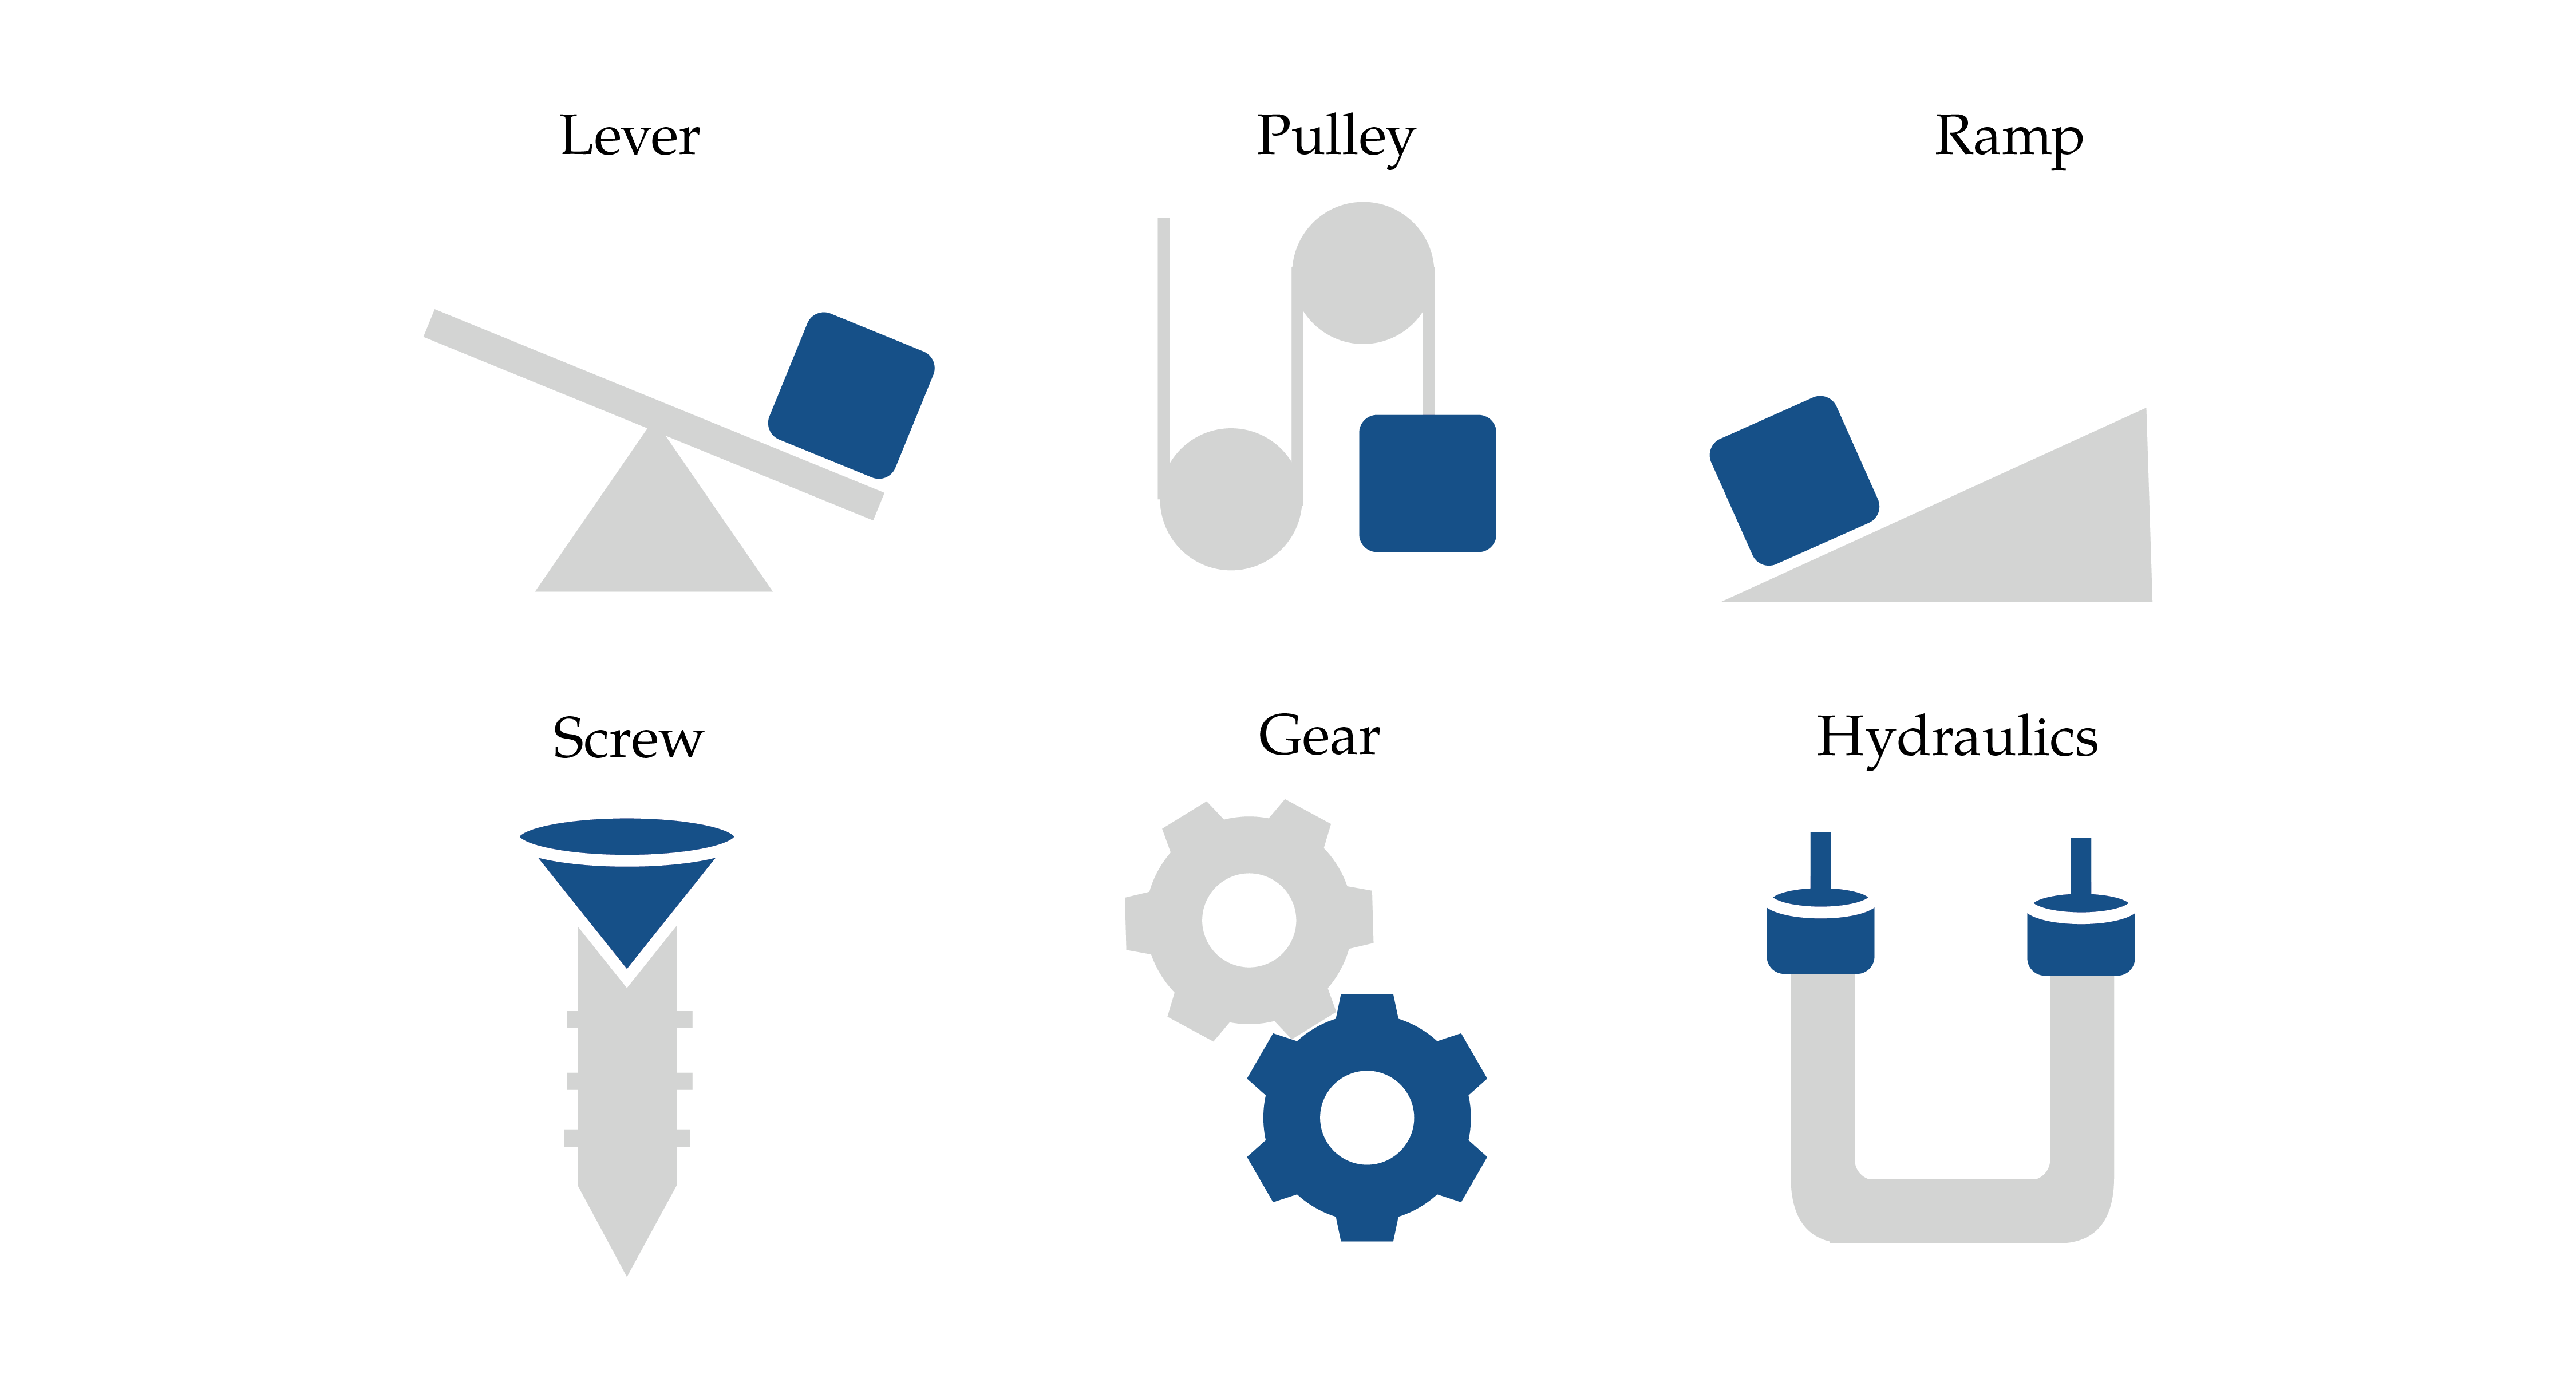
\includegraphics[width=0.6\textwidth]{simplemachines.png}

While these machines can decrease the force needed, they don't change
the amount of work that must be done. So if the force is decreased to
a third, the distance that you must apply the force is increased by a
factor of three.

``Mechanical gain'' is what we call the increase in force.

\section{Levers}

A lever rotates on a fulcrum. To decrease the necessary force, the load
is placed nearer to the fulcrum than where the force is applied.

In particular, physicists talk about the \newterm{torque} created by a
force. When you push on a lever, the torque is the product of the
force you exert and the distance from the point of rotation.

Torque is typically measured in newton-meters.

To balance two torques, the products must be the same. So, assuming
that the forces are applied in the proper direction,

$$R_L F_L = R_A F_A$$

where $R_L$ and $R_A$ are the distance from the fulcrum to the where
the load's force and the applied force (respectively) are applied, and
$F_L$ and $F_A$ are the amounts of the forces.

\begin{Exercise}[title={Lever}, label=lever]
  
Paul, who weighs 70 kilograms, sits on a see-saw 4 meters from the
fulcrum. Jan, who weighs 50 kilograms, wants to balance. How far
should Jan sit from the fulcrum?

\end{Exercise}
\begin{Answer}[ref=lever]
  Paul is exerting $(70)(9.8)$ newtons of force at 4 meters from the
  fulcrum, so he is creating a torque of 2,744 newton-meters of torque
  on the see-saw.  Jan is creating $(50)(9.5) = 490$ newtons of
  force.

  If $r$ is the distance from the fulcrum to Jan's seat, to balance
  $490 r = 2744$, so $r = 5.6$ meters.
\end{Answer}

Watch Khan Academy's video on levers: \url{https://www.khanacademy.org/science/physics/discoveries/simple-machines-explorations/a/lever}

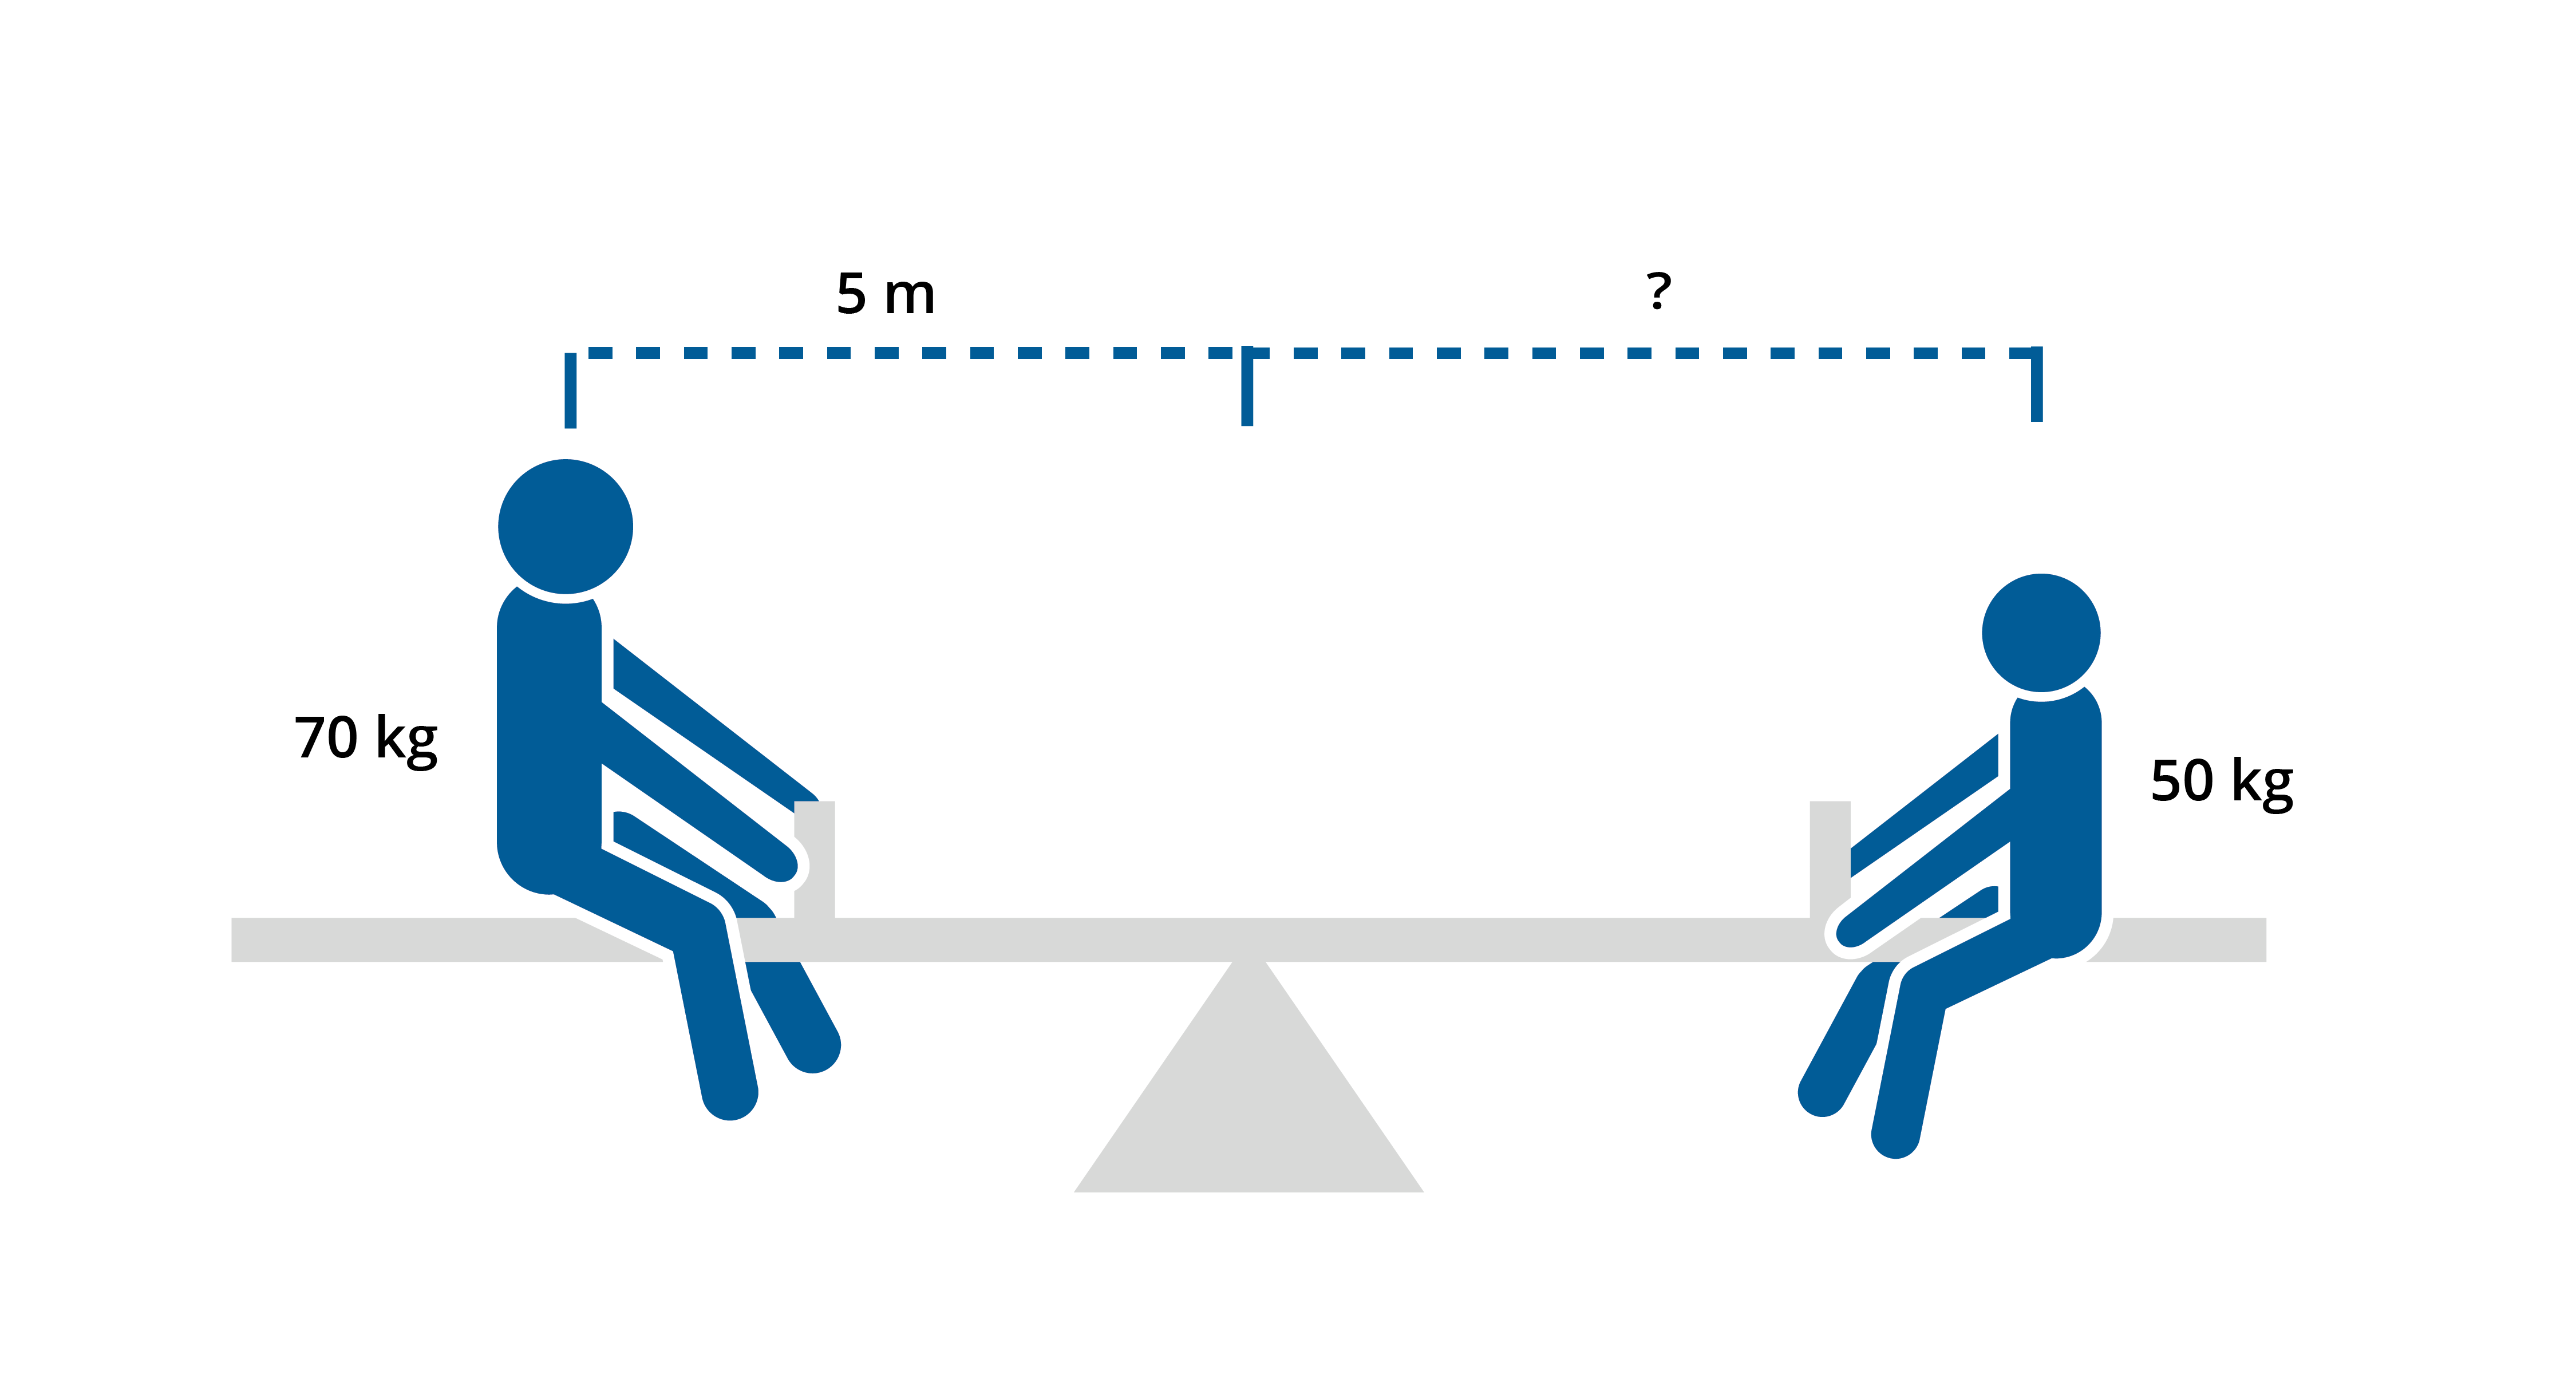
\includegraphics[width=1\textwidth]{seesaw.png}

\section{Ramps}

Ramps, or incline planes, let you roll or slide objects up to a higher
level. Steeper ramps give you less mechanical gain. For example, it is much easier 
to roll a ball up a wheelchair ramp than on a skateboard ramp.
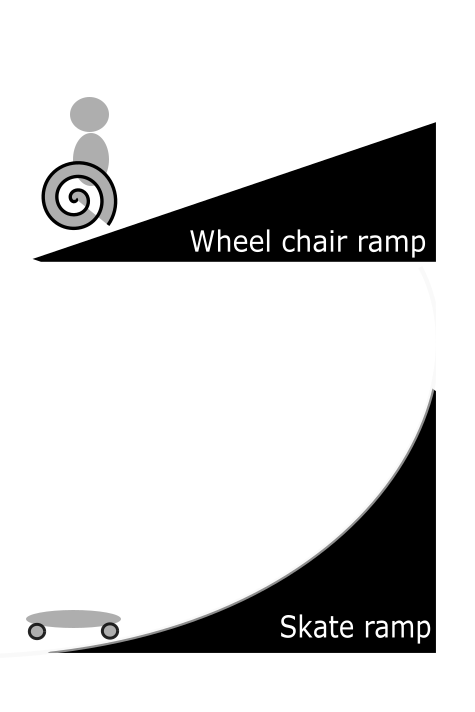
\includegraphics[width=0.6\textwidth]{ramps.png}

Assuming the ramp has a constant steepness, the mechanical gain is
equal to the ratio of the length of the ramp divided by the amount
that it rises.

If you assume there is no friction, the force that you push a weight up the ramp will be:

$$F_A = \frac{V}{L} F_G$$

Where $F_A$ is the force you need to push. $L$ is the length of the
ramp, $V$ is the amount of vertical gain and $F_G$ is the force of
gravity on the mass.

(We haven't talked about the sine function yet, but in case you already know about it: Note that

$$\frac{V}{L} = \sin{\theta}$$

where $\theta$ is the angle between the ramp and level.)

\begin{Exercise}[title={Ramp}, label=ramp]
A barrel of oil weighs 136 kilograms. You can push with a force of
up to 300 newtons. You have to get the barrel onto a platform that is 2
meters. What is the shortest board that you can use as a ramp?
\end{Exercise}
\begin{Answer}[ref=ramp]
  To lift the barrel would require $136 \times 9.8 = 1,332.8$ newtons of force.

  Letting $L$ be the length of the ramp:

  $$300= \frac{2}{L} 1332.8$$

  So $L = 8.885$ meters.
\end{Answer}

\section{Gears}

Gears (which might have a chain connecting them like on a bicycle)
have teeth and come in pairs. You apply torque to one gear, and it
applies torque to another. The torque is increased or decreased based
on the ratio between the teeth on the gears.


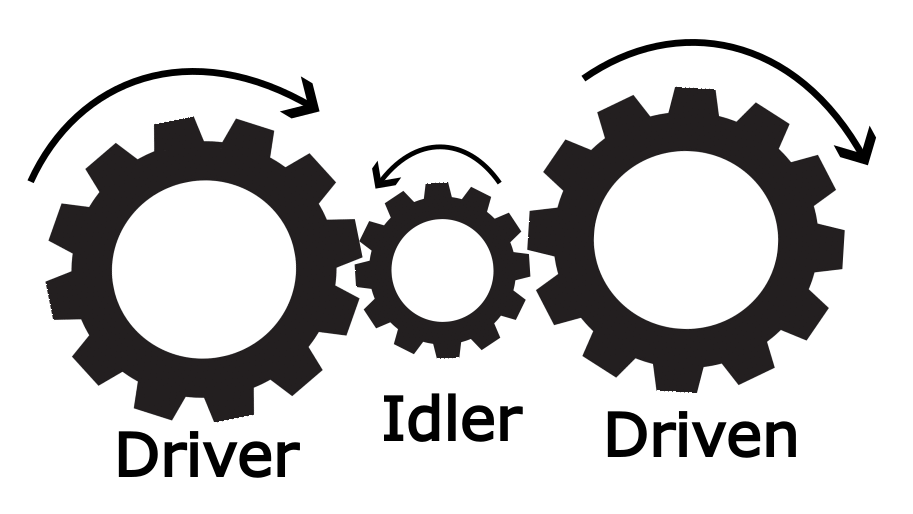
\includegraphics[width=0.6\textwidth]{Gears.png}


If $N_A$ is the number of teeth on the gear you are turning with a
torque of $T_A$, and $N_L$ is the number of teeth on the gear it is
turning, the resulting torque is:

$$T_L = \frac{N_A}{N_L} T_A$$


\begin{Exercise}[title={Gears}, label=gear]

The bicycle is an interesting case because we are not trying to get
mechanical gain. We want to spin the pedals slower with more force.
  
You like to pedal your bike at 70 revolutions per minute. The
chainring that is connected to your pedals has 53 teeth. The
circumference of your tire is 2.2 meters. You wish to ride a 583 meters
per minute.

How many teeth should the rear sprocket have?
  
\end{Exercise}
\begin{Answer}[ref=ramp]
  
  $$583 = (70)(2.2)\frac{53}{n}$$
  
Thus $n = 14$ teeth.
\end{Answer}

Watch Khan Academy's introduction to simple machines here: \url{https://www.khanacademy.org/science/physics/discoveries/simple-machines-explorations/a/simple-machines-and-how-to-use-this-tutorial}

\section{Hydraulics}

In a hydraulic system, like the braking system of a car, you exert
force on a piston filled with fluid. The fluid carries that pressure
into another cylinder. The pressure of the fluid pushes the piston in
that cylinder out.

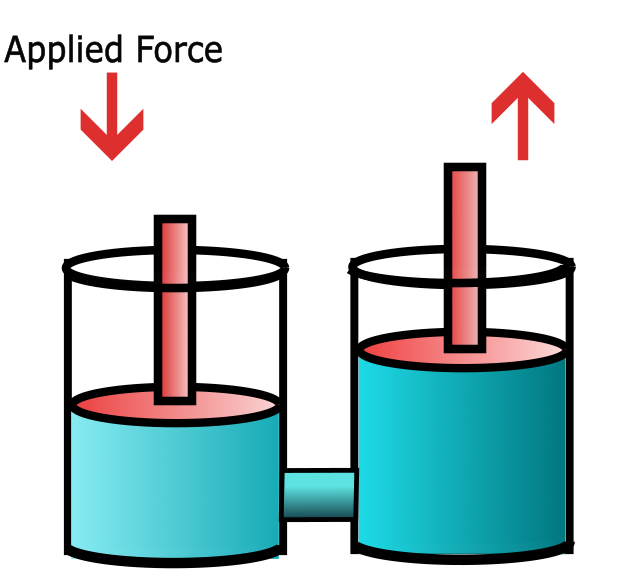
\includegraphics[width=0.6\textwidth]{hydraulics.png}


The pressure in the hose can be measured in pounds per square inch
(PSI) or newtons per square meter (Pascals or Pa). We will use Pascals.
% ADD: Create a page in the back of the book with units

To figure out how much pressure you create, you divide the force by
the area of the piston head you are pushing.

To figure out how much force that creates on the other end, you
multiply the pressure times the area of the piston head that is
pushing the load.

\begin{Exercise}[title={Hydraulics}, label=hydraulics]

Your car has disc brakes. When you put 2,500,000 pascals of pressure on the
brake fluid, the car stops quickly. As the car designer, you would like
that to require 12 newtons of force from the driver's foot.

What should the radius of the master cylinder (the one the driver is pushing on) be?
\end{Exercise}
\begin{Answer}[ref=hydraulics]
  We are looking for $r$, the radius of the piston head in meters. The area of the piston head is $\pi r^2$.

  The pressure in pascals of the brake fluid is given by $12 / (\pi r^2)$.

  $$2,500,000 = \frac{12}{\pi r^2}$$

  So $r = \sqrt{\frac{12}{\pi \times 2.5 \times 10^6}} = 0.001236077446474$ meters.

\end{Answer}
% KA: https://youtu.be/Pn5YEMwQb4Y



\graphicspath{{../../Chapters/buoyancy/en_US}}
\chapter{Buoyancy}

When you put a boat into water, it will sink into the water until
the mass of the water it displaces is equal to the mass of the
boat. We think of this in terms of forces. Gravity pulls the mass of
the boat down. The \newterm{buoyant force} pushes the boat up. A boat
dropped into the water will bob up and down a bit before reaching an
equilibrium where the two forces are equal.
% ADD: Explain Action Reaction Pairs in previous chapter
% ADD: Archimedes principle

Watch Khan Academy's introduction to buoyance at \url{https://www.khanacademy.org/science/in-in-class9th-physics-india/in-in-gravity/in-in-pressure-in-liquids-archimedes-principle/v/archimedes-principle-buoyancy-fluids-physics-khan-academy}

The buoyant force pushes things up -- against the force of
gravity. The force is equal to the weight of the fluid being
replaced. So, for example, a cubic meter of freshwater has a mass of
about 1000kg.  If you submerge anything with a volume of one meter in
freshwater on earth, the buoyant force will be about 9800 newtons.

For some things, like a block of styrofoam, this buoyant force will be
sufficient to carry it to the surface. Once it reaches the surface, it
will continue to rise (displacing less water) until the mass of the
water it displaces is equal to its mass. And then we say ``It floats!''

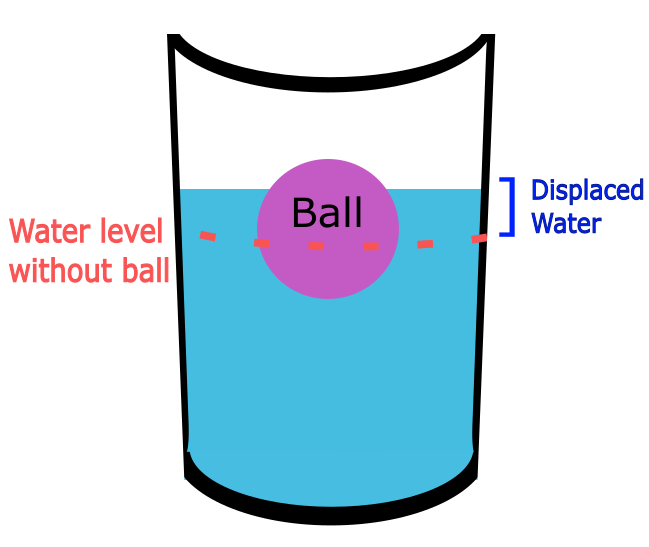
\includegraphics[width=0.5\textwidth]{Buoyancy_Displacement_Diagram.png}

For some things, like a block of lead, the buoyant force is not
 sufficient to lift it to the surface, and thus we say ``It sinks!''

This is why a helium balloon floats through the air. The air
that it displaces weighs more than the balloon and the helium itself. (It is easy to forget that air has a mass, but it does.)

\begin{Exercise}[title={Buoyancy}, label=buoyancy]
  You have an aluminum box that has a heavy base, so it will always
  float upright. The box and its contents weigh 10 kg. Its base is 0.3 m x 0.4 m. It is 1m tall.

  When you drop it into freshwater ($1000 kg/m^3$), how far will it sink
  before it reaches equilibrium.
  
\end{Exercise}
\begin{Answer}[ref=buoyancy]
  Equilibrium will be achieved when the box has displaced 10 kg of water. That is, when it has displaced $0.01$ cubic meters.

  The area of the base of the box is 0.12 square meters.  So if the
  box sinks $x$ meters into the water it will displace $0.12 x$ cubic
  meters.

  Thus at equilibrium $x = \frac{0.01}{0.12} \approx 0.083$ m.  So,
  the box will sink 8.3 cm into the water before reaching equilibrium.
\end{Answer}

\section{The Mechanism of Buoyancy}

As you dive down in the ocean, you will experience greater and
greater pressure from the water. And if you take a balloon with you, you
will gradually see it get smaller as the water pressure compresses the
air in the balloon.

Let's say you are 3 meters below the surface of the water. What is the
pressure in Pascals (newtons per square meter)? You can think of the
water as a column of water crushing down upon you. The pressure over
a square meter is the weight of 3 cubic meters of water pressing down.

$$p = (3)(1000)(9.8) = 29,400 \text{ Pa }$$

This is called \newterm{hydrostatic pressure}. The general rule for
hydrostatic pressure in Pascals $p$ is

$p = d g h$

Where  $d$ is the density of the fluid
in kg per cubic meter, $g$ is the acceleration due to gravity in
$m/s^2$, and $h$ is the height of the column of fluid above you.

So, where does buoyant force come from? Basically, the pressure pushing up on the
deepest part of the object is higher than the pressure pushing down on
the shallowest part of the object. That is where bouyancy comes from.

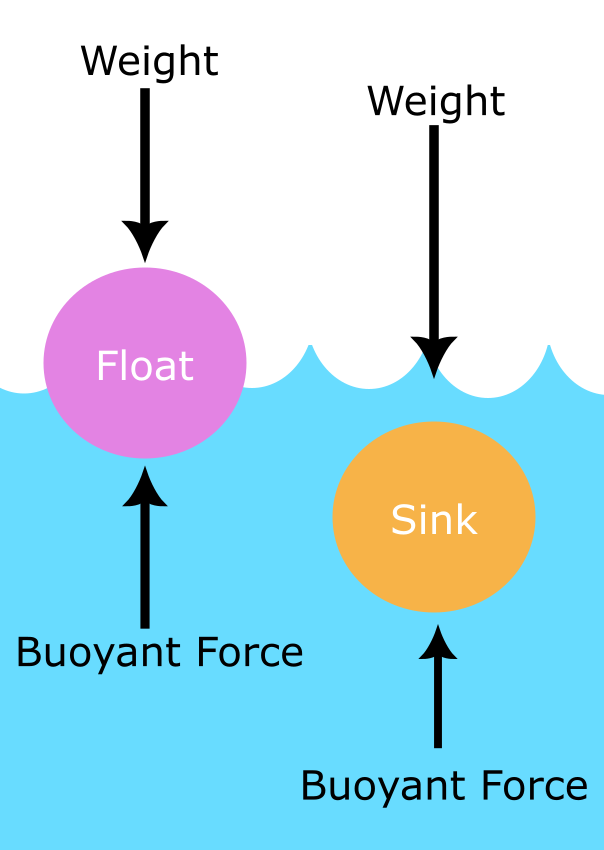
\includegraphics[width=0.5\textwidth]{Buoyancy_Diagram.png}

\begin{Exercise}[title={Hydrostatic Pressure}, label=mars_pressure]

  You dive into a tank of olive oil on Mars. How much more
  hydrostatic pressure does your body experience at 5 meters deep than
  it did at the surface?

  The density of olive oil is about 900 kg per square meter. The
  acceleration due to gravity on Mars is 3.721 $m/s^2$.
  
\end{Exercise}
\begin{Answer}[ref=mars_pressure]
$$p = d g h = (900)(3.721)(5) = 16,744.5 \text{ Pa}$$
\end{Answer}

Notice that although the pressure is increasing as you go deeper, the
buoyant force will \emph{not increase} because the buoyant force is always equal
to the weight of the fluid that is displaced, regardless if that is 1
meter or 100 meters underwater.

Also, saltwater is denser then freshwater. That is why people float
better in the sea than they do in a river.

And, lipids, like fats and oils, are less dense than water. That is why
people with a lot of body fat tend to float better than people with
less body fat. And why oil floats in a glass of water.


\graphicspath{{../../Chapters/heat/en_US}}
\chapter{Heat}

Let's say you put a 1 kg aluminum pan that is $80^\circ$ C into
3 liters of water that is $20^\circ$ C. Energy, in the form of heat,
will be transferred from the pan to the water until they are at the same
temperature. (We call this ``thermal equilibrium.'')\index{thermal equilibrium}

What will the temperature of the water be?

\section{Specific Heat Capacity}

If you are heating something, the amount of energy you need to
transfer to it depends on three things: the mass of the thing you are
heating, the amount of temperature change you want, and the
\textit{specific heat capacity} of that substance.\index{specific heat capacity}

\begin{mdframed}[style=important, frametitle={Energy in Heat Transfer}]

  The energy moved in a heat transfer is given by

  $$E = m c \Delta_T$$

  where $m$ is the mass, $\Delta_T$ is the change in temperature, and
  $c$ is the specific heat capacity of the substance.
% ADD: q=mcat

  (Note that this
  assumes no phase change. For example, this formula works nicely on
  warming liquid water, but it gets more complicated if you warm the
  water past its boiling point.)

\end{mdframed}

Can we guess the specific heat capacity of a substance? It is very,
very difficult to guess the specific heat of a substance, so we determine
it by experimentation.

For example, someone determined that it took about 0.9 joules to raise
the temperature of solid aluminum one degree Celsius. So we say ``The
specific heat capacity of aluminum is 0.9 J/g $^\circ$C.''

The specific heat capacity of liquid water is about 4.2 J/g $^\circ$C.

To answer the question, then, the amount of energy given off by the
pan must equal the amount of energy absorbed by the water. And they
need to be the same temperature at the end.  Let $T$ be the final
temperature of both.

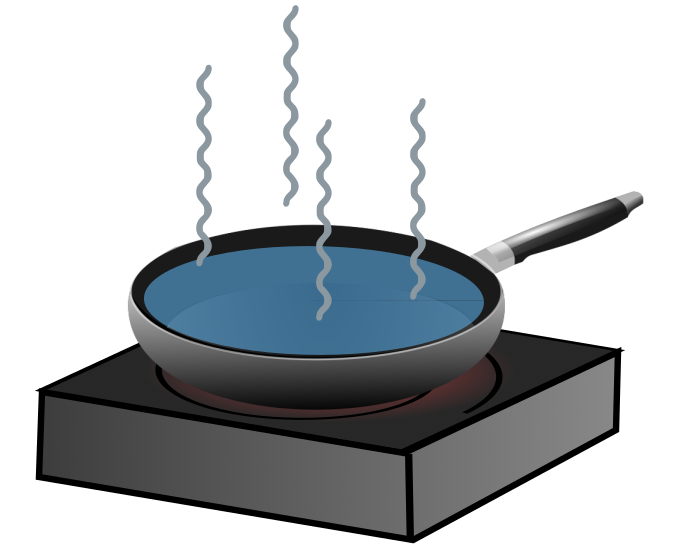
\includegraphics[width=0.5\textwidth]{pan.png}

Watch Khan Academy's discussion of heat capacity at \url{https://www.khanacademy.org/science/ap-chemistry-beta/x2eef969c74e0d802:thermodynamics/x2eef969c74e0d802:heat-capacity-and-calorimetry/v/heat-capacity}


Three liters of water weighs 3,000 grams, so the
change in energy in the water will be:

$$E_W = m c \Delta_T = (3000)(4.2)(T - 20) = 12600T - 252000 \text{ joules}$$ 

The pan weighs 1000 grams, so the change in energy in the pan will be::

$$E_P = m c \Delta_T = (1000)(0.9)(T - 80) = 900T - 72000 \text{ joules}$$

Total energy stays the same so $E_W + E_P = 0$.  So you need to solve

$$(12600T - 252000) + (900T - 72000) = 0$$

And find that the temperature at equilibrium will be

$$T = 24^\circ \text{C}$$

\begin{Exercise}[title={Thermal Equilibrium}, label=thermal_equilibrium]

Just as you put the aluminium pan in the water as described above,
someone also puts a 1.2 kg block of copper cooled to 10 $^\circ$ C.
The specific heat of solid copper is about 0.4 J/g $^\circ$C.

What is the new temperature at equilibrium?

\end{Exercise}
\begin{Answer}[ref=thermal_equilibrium]

  $$E_C = (1200)(0.4)(T - 10) = 480T - 4800$$

Total energy stays constant:

$$0 = (12600T - 252000) + (900T - 72000) + (480T - 4800)$$

Solving for $T$ gets you $T = 23.52^\circ$ C.

\end{Answer}

\section{Getting to Equilibrium}

When two objects with different temperatures are touching, the speed
at which they exchange heat is proportional to the differences in
their temperatures. Thus, as their temperatures get closer together,
the heat exchange slows down.
% ADD: explain which object, water or metal has a greater tempature change

In our example, the pan and the water will get close to equilibrium
quickly, but they may never actually reach equilibrium.

\begin{tikzpicture}
    \begin{axis}[
        xmin=0,xmax=4.25,
        ymin=15,ymax=85,
        axis x line=middle,
        axis y line=middle,
        axis line style=<->,
        xlabel={minutes},
        ylabel={degrees celsius},
        ]
        \addplot[no marks,sdkblue] expression[domain=0:4,samples=100]{24 + 56 * pow(2,-1.5 * x)} node[above, xshift=-1cm, yshift=0.1cm]{Pan}; 
        \addplot[no marks,sdkblue] expression[domain=0:4,samples=100]{24 - 4 * pow(2,-0.8 * x)} node[below, xshift=-2.5cm]{Water};
        \addplot[no marks,dashed,gray] coordinates {(0,24)(6,24)} node[above, xshift=-8cm]{equilibrium};
    \end{axis}
\end{tikzpicture}

\begin{Exercise}[title={Cooling Your Coffee}, label=cool_coffee]

  You have been given a ridiculously hot cup of coffee and a small pitcher of chilled milk.

  You need to start chugging your coffee in three minutes, and you want it as cool as possible at that time. When should you add the milk to the coffee?

\end{Exercise}
\begin{Answer}[ref=cool_coffee]

  During the 3 minutes, you want the coffee to give off as much of its
  heat as possible, so you want to maximize the difference between the
  temperature of the coffee and the temperature of the room around
  it.

  You wait until the last moment to put the milk in.

\end{Answer}

\section{Specific Heat Capacity Details}

For any given substance, the specific heat capacity often changes a
lot when the substance changes state. For example, ice is 2.1 J/g
$^\circ$C, whereas liquid water is 4.2 J/g$^\circ$C.

Watch Khan Academy's discussion of the specific heat of water: \url{https://www.khanacademy.org/science/biology/water-acids-and-bases/water-as-a-solid-liquid-and-gas/v/specific-heat-of-water}

Even within a given state, the specific heat capacity varies a bit
based on the temperature and pressure. If you are trying to do these
sorts of calculations with great accuracy, you will want to find the
specific heat capacity that matches your situation. For example, I
might look for the specific heat capacity for water at $22^\circ$C at
1 atmosphere of pressure( atm).


%%%%%%%%%%%%%%%%%%%%%%%%%%%%%%%%%
%% Bookfooter.tex by Aaron Hillegass
%% Nov 8, 2020

\appendix

\chapter{Answers to Exercises}
\shipoutAnswer

\bibliography{references}

\printindex

\end{document}